% Options for packages loaded elsewhere
\PassOptionsToPackage{unicode}{hyperref}
\PassOptionsToPackage{hyphens}{url}
%
\documentclass[
]{article}
\usepackage{amsmath,amssymb}
\usepackage{iftex}
\ifPDFTeX
  \usepackage[T1]{fontenc}
  \usepackage[utf8]{inputenc}
  \usepackage{textcomp} % provide euro and other symbols
\else % if luatex or xetex
  \usepackage{unicode-math} % this also loads fontspec
  \defaultfontfeatures{Scale=MatchLowercase}
  \defaultfontfeatures[\rmfamily]{Ligatures=TeX,Scale=1}
\fi
\usepackage{lmodern}
\ifPDFTeX\else
  % xetex/luatex font selection
\fi
% Use upquote if available, for straight quotes in verbatim environments
\IfFileExists{upquote.sty}{\usepackage{upquote}}{}
\IfFileExists{microtype.sty}{% use microtype if available
  \usepackage[]{microtype}
  \UseMicrotypeSet[protrusion]{basicmath} % disable protrusion for tt fonts
}{}
\makeatletter
\@ifundefined{KOMAClassName}{% if non-KOMA class
  \IfFileExists{parskip.sty}{%
    \usepackage{parskip}
  }{% else
    \setlength{\parindent}{0pt}
    \setlength{\parskip}{6pt plus 2pt minus 1pt}}
}{% if KOMA class
  \KOMAoptions{parskip=half}}
\makeatother
\usepackage{xcolor}
\usepackage[margin=1in]{geometry}
\usepackage{color}
\usepackage{fancyvrb}
\newcommand{\VerbBar}{|}
\newcommand{\VERB}{\Verb[commandchars=\\\{\}]}
\DefineVerbatimEnvironment{Highlighting}{Verbatim}{commandchars=\\\{\}}
% Add ',fontsize=\small' for more characters per line
\usepackage{framed}
\definecolor{shadecolor}{RGB}{248,248,248}
\newenvironment{Shaded}{\begin{snugshade}}{\end{snugshade}}
\newcommand{\AlertTok}[1]{\textcolor[rgb]{0.94,0.16,0.16}{#1}}
\newcommand{\AnnotationTok}[1]{\textcolor[rgb]{0.56,0.35,0.01}{\textbf{\textit{#1}}}}
\newcommand{\AttributeTok}[1]{\textcolor[rgb]{0.13,0.29,0.53}{#1}}
\newcommand{\BaseNTok}[1]{\textcolor[rgb]{0.00,0.00,0.81}{#1}}
\newcommand{\BuiltInTok}[1]{#1}
\newcommand{\CharTok}[1]{\textcolor[rgb]{0.31,0.60,0.02}{#1}}
\newcommand{\CommentTok}[1]{\textcolor[rgb]{0.56,0.35,0.01}{\textit{#1}}}
\newcommand{\CommentVarTok}[1]{\textcolor[rgb]{0.56,0.35,0.01}{\textbf{\textit{#1}}}}
\newcommand{\ConstantTok}[1]{\textcolor[rgb]{0.56,0.35,0.01}{#1}}
\newcommand{\ControlFlowTok}[1]{\textcolor[rgb]{0.13,0.29,0.53}{\textbf{#1}}}
\newcommand{\DataTypeTok}[1]{\textcolor[rgb]{0.13,0.29,0.53}{#1}}
\newcommand{\DecValTok}[1]{\textcolor[rgb]{0.00,0.00,0.81}{#1}}
\newcommand{\DocumentationTok}[1]{\textcolor[rgb]{0.56,0.35,0.01}{\textbf{\textit{#1}}}}
\newcommand{\ErrorTok}[1]{\textcolor[rgb]{0.64,0.00,0.00}{\textbf{#1}}}
\newcommand{\ExtensionTok}[1]{#1}
\newcommand{\FloatTok}[1]{\textcolor[rgb]{0.00,0.00,0.81}{#1}}
\newcommand{\FunctionTok}[1]{\textcolor[rgb]{0.13,0.29,0.53}{\textbf{#1}}}
\newcommand{\ImportTok}[1]{#1}
\newcommand{\InformationTok}[1]{\textcolor[rgb]{0.56,0.35,0.01}{\textbf{\textit{#1}}}}
\newcommand{\KeywordTok}[1]{\textcolor[rgb]{0.13,0.29,0.53}{\textbf{#1}}}
\newcommand{\NormalTok}[1]{#1}
\newcommand{\OperatorTok}[1]{\textcolor[rgb]{0.81,0.36,0.00}{\textbf{#1}}}
\newcommand{\OtherTok}[1]{\textcolor[rgb]{0.56,0.35,0.01}{#1}}
\newcommand{\PreprocessorTok}[1]{\textcolor[rgb]{0.56,0.35,0.01}{\textit{#1}}}
\newcommand{\RegionMarkerTok}[1]{#1}
\newcommand{\SpecialCharTok}[1]{\textcolor[rgb]{0.81,0.36,0.00}{\textbf{#1}}}
\newcommand{\SpecialStringTok}[1]{\textcolor[rgb]{0.31,0.60,0.02}{#1}}
\newcommand{\StringTok}[1]{\textcolor[rgb]{0.31,0.60,0.02}{#1}}
\newcommand{\VariableTok}[1]{\textcolor[rgb]{0.00,0.00,0.00}{#1}}
\newcommand{\VerbatimStringTok}[1]{\textcolor[rgb]{0.31,0.60,0.02}{#1}}
\newcommand{\WarningTok}[1]{\textcolor[rgb]{0.56,0.35,0.01}{\textbf{\textit{#1}}}}
\usepackage{graphicx}
\makeatletter
\def\maxwidth{\ifdim\Gin@nat@width>\linewidth\linewidth\else\Gin@nat@width\fi}
\def\maxheight{\ifdim\Gin@nat@height>\textheight\textheight\else\Gin@nat@height\fi}
\makeatother
% Scale images if necessary, so that they will not overflow the page
% margins by default, and it is still possible to overwrite the defaults
% using explicit options in \includegraphics[width, height, ...]{}
\setkeys{Gin}{width=\maxwidth,height=\maxheight,keepaspectratio}
% Set default figure placement to htbp
\makeatletter
\def\fps@figure{htbp}
\makeatother
\setlength{\emergencystretch}{3em} % prevent overfull lines
\providecommand{\tightlist}{%
  \setlength{\itemsep}{0pt}\setlength{\parskip}{0pt}}
\setcounter{secnumdepth}{-\maxdimen} % remove section numbering
\usepackage{booktabs}
\usepackage{caption}
\usepackage{longtable}
\usepackage{colortbl}
\usepackage{array}
\usepackage{anyfontsize}
\usepackage{multirow}
\usepackage{graphicx}
\usepackage{siunitx}
\usepackage[normalem]{ulem}
\usepackage{hhline}
\usepackage{calc}
\usepackage{tabularx}
\usepackage{threeparttable}
\usepackage{wrapfig}
\usepackage{adjustbox}
\usepackage{hyperref}
\usepackage{float}
\usepackage{pdflscape}
\usepackage{tabu}
\usepackage{threeparttablex}
\usepackage{makecell}
\usepackage{xcolor}
\ifLuaTeX
  \usepackage{selnolig}  % disable illegal ligatures
\fi
\usepackage{bookmark}
\IfFileExists{xurl.sty}{\usepackage{xurl}}{} % add URL line breaks if available
\urlstyle{same}
\hypersetup{
  pdftitle={Assignment 1: California Spiny Lobster Abundance (Panulirus Interruptus)},
  pdfauthor={Kaiju Morquecho},
  hidelinks,
  pdfcreator={LaTeX via pandoc}}

\title{Assignment 1: California Spiny Lobster Abundance (\emph{Panulirus
Interruptus})}
\usepackage{etoolbox}
\makeatletter
\providecommand{\subtitle}[1]{% add subtitle to \maketitle
  \apptocmd{\@title}{\par {\large #1 \par}}{}{}
}
\makeatother
\subtitle{Assessing the Impact of Marine Protected Areas (MPAs) at 5
Reef Sites in Santa Barbara County}
\author{Kaiju Morquecho}
\date{1/8/2024 (Due 1/26)}

\begin{document}
\maketitle

\begin{center}\rule{0.5\linewidth}{0.5pt}\end{center}

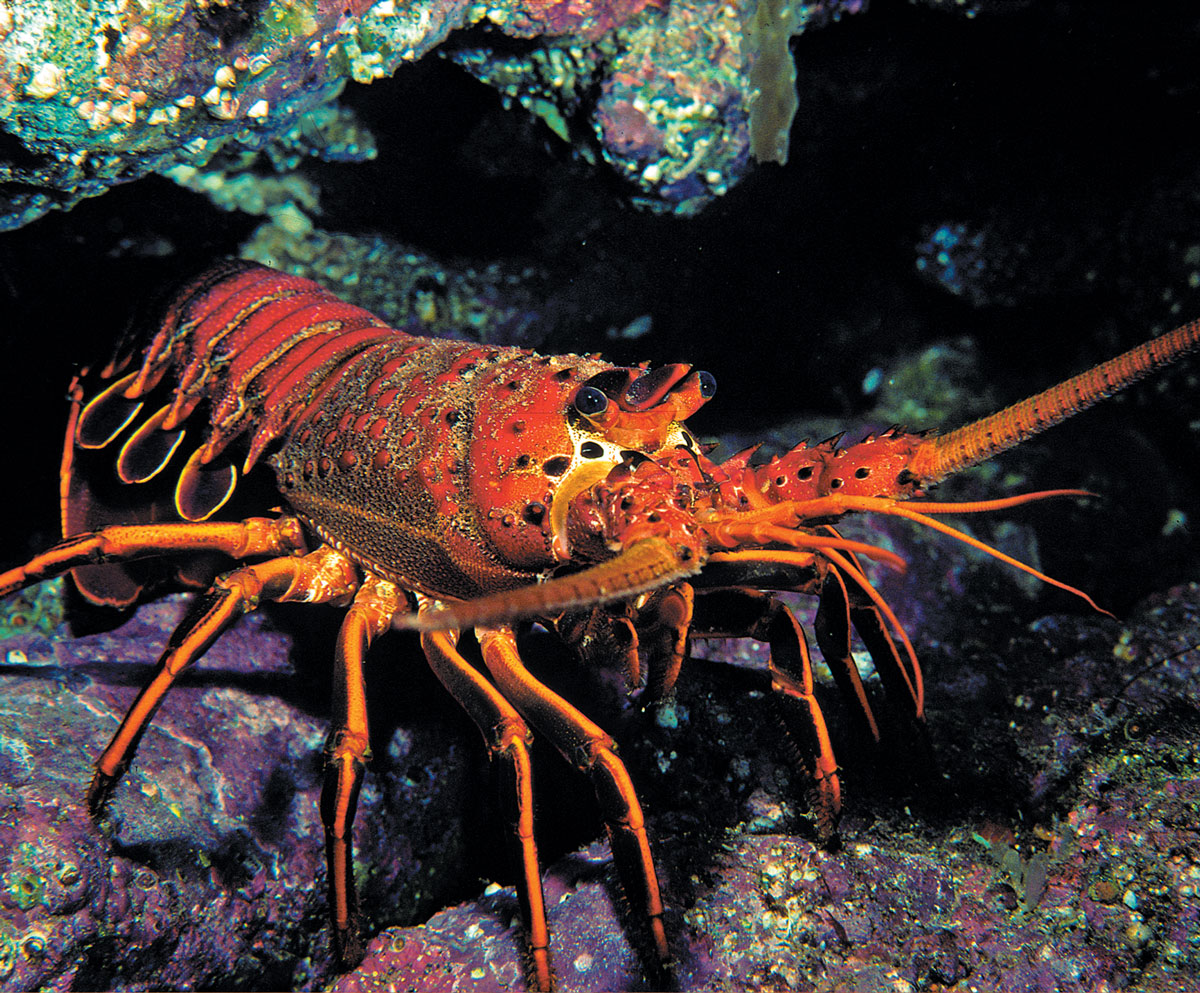
\includegraphics{figures/spiny2.jpg}

\begin{center}\rule{0.5\linewidth}{0.5pt}\end{center}

\subsubsection{Assignment instructions:}\label{assignment-instructions}

\begin{itemize}
\item
  Working with partners to troubleshoot code and concepts is encouraged!
  If you work with a partner, please list their name next to yours at
  the top of your assignment so Annie and I can easily see who
  collaborated.
\item
  All written responses must be written independently (\textbf{in your
  own words}).
\item
  Please follow the question prompts carefully and include only the
  information each question asks in your submitted responses.
\item
  Submit both your knitted document and the associated
  \texttt{RMarkdown} or \texttt{Quarto} file.
\item
  Your knitted presentation should meet the quality you'd submit to
  research colleagues or feel confident sharing publicly. Refer to the
  rubric for details about presentation standards.
\end{itemize}

\textbf{Assignment submission (YOUR NAME):} \textbf{\emph{Kaiju
Morquecho }}

\begin{center}\rule{0.5\linewidth}{0.5pt}\end{center}

\begin{Shaded}
\begin{Highlighting}[]
\FunctionTok{library}\NormalTok{(tidyverse)}
\end{Highlighting}
\end{Shaded}

\begin{verbatim}
## -- Attaching core tidyverse packages ------------------------ tidyverse 2.0.0 --
## v dplyr     1.1.4     v readr     2.1.5
## v forcats   1.0.0     v stringr   1.5.1
## v ggplot2   3.5.1     v tibble    3.2.1
## v lubridate 1.9.3     v tidyr     1.3.1
## v purrr     1.0.2     
## -- Conflicts ------------------------------------------ tidyverse_conflicts() --
## x dplyr::filter() masks stats::filter()
## x dplyr::lag()    masks stats::lag()
## i Use the conflicted package (<http://conflicted.r-lib.org/>) to force all conflicts to become errors
\end{verbatim}

\begin{Shaded}
\begin{Highlighting}[]
\FunctionTok{library}\NormalTok{(here)}
\end{Highlighting}
\end{Shaded}

\begin{verbatim}
## here() starts at /Users/kaiju/MEDS/EDS241/EDS241_HW1
\end{verbatim}

\begin{Shaded}
\begin{Highlighting}[]
\FunctionTok{library}\NormalTok{(janitor)}
\end{Highlighting}
\end{Shaded}

\begin{verbatim}
## 
## Attaching package: 'janitor'
## 
## The following objects are masked from 'package:stats':
## 
##     chisq.test, fisher.test
\end{verbatim}

\begin{Shaded}
\begin{Highlighting}[]
\FunctionTok{library}\NormalTok{(estimatr)  }
\FunctionTok{library}\NormalTok{(performance)}
\FunctionTok{library}\NormalTok{(jtools)}
\FunctionTok{library}\NormalTok{(gt)}
\FunctionTok{library}\NormalTok{(gtsummary)}
\FunctionTok{library}\NormalTok{(MASS) }\DocumentationTok{\#\# }\AlertTok{NOTE}\DocumentationTok{: The \textasciigrave{}select()\textasciigrave{} function is masked. Use: \textasciigrave{}dplyr::select()\textasciigrave{} \#\#}
\end{Highlighting}
\end{Shaded}

\begin{verbatim}
## 
## Attaching package: 'MASS'
## 
## The following object is masked from 'package:gtsummary':
## 
##     select
## 
## The following object is masked from 'package:dplyr':
## 
##     select
\end{verbatim}

\begin{Shaded}
\begin{Highlighting}[]
\FunctionTok{library}\NormalTok{(interactions) }
\FunctionTok{library}\NormalTok{(ggridges)}
\FunctionTok{library}\NormalTok{(ggrepel)}
\FunctionTok{library}\NormalTok{(dplyr)}
\end{Highlighting}
\end{Shaded}

\begin{center}\rule{0.5\linewidth}{0.5pt}\end{center}

\paragraph{DATA SOURCE:}\label{data-source}

Reed D. 2019. SBC LTER: Reef: Abundance, size and fishing effort for
California Spiny Lobster (Panulirus interruptus), ongoing since 2012.
Environmental Data Initiative.
\url{https://doi.org/10.6073/pasta/a593a675d644fdefb736750b291579a0}.
Dataset accessed 11/17/2019.

\begin{center}\rule{0.5\linewidth}{0.5pt}\end{center}

\subsubsection{\texorpdfstring{\textbf{Introduction}}{Introduction}}\label{introduction}

You're about to dive into some deep data collected from five reef sites
in Santa Barbara County, all about the abundance of California spiny
lobsters! Data was gathered by divers annually from 2012 to 2018 across
Naples, Mohawk, Isla Vista, Carpinteria, and Arroyo Quemado reefs.

Why lobsters? Well, this sample provides an opportunity to evaluate the
impact of Marine Protected Areas (MPAs) established on January 1, 2012
(Reed, 2019). Of these five reefs, Naples, and Isla Vista are MPAs,
while the other three are not protected (non-MPAs). Comparing lobster
health between these protected and non-protected areas gives us the
chance to study how commercial and recreational fishing might impact
these ecosystems.

We will consider the MPA sites the \texttt{treatment} group and use
regression methods to explore whether protecting these reefs really
makes a difference compared to non-MPA sites (our control group). In
this assignment, we'll think deeply about which causal inference
assumptions hold up under the research design and identify where they
fall short.

Let's break it down step by step and see what the data reveals!

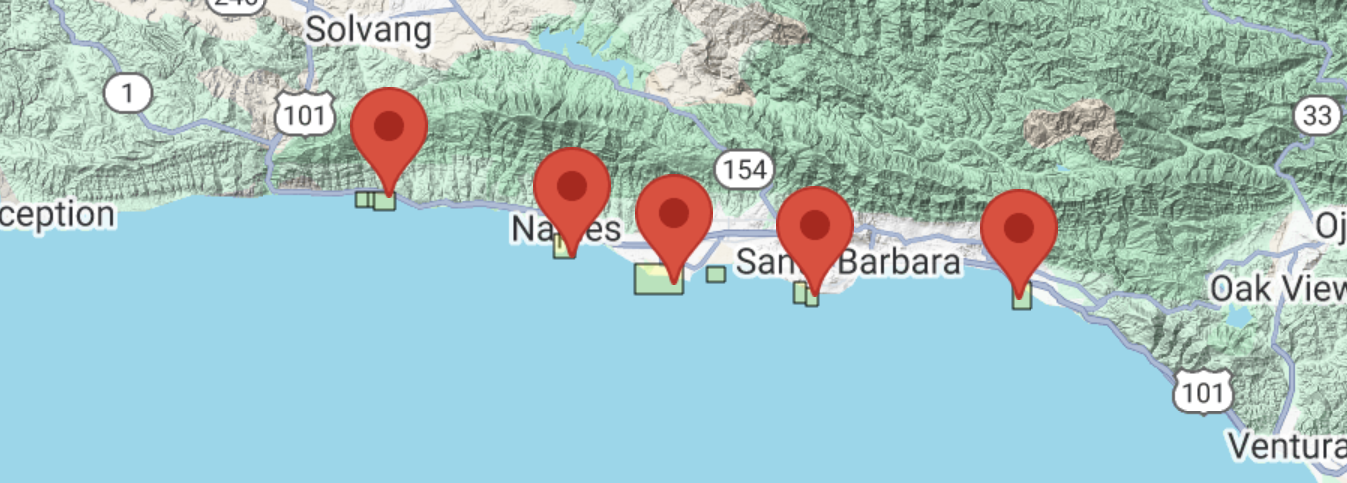
\includegraphics{figures/map-5reefs.png}

\begin{center}\rule{0.5\linewidth}{0.5pt}\end{center}

Step 1: Anticipating potential sources of selection bias

\textbf{a.} Do the control sites (Arroyo Quemado, Carpenteria, and
Mohawk) provide a strong counterfactual for our treatment sites (Naples,
Isla Vista)? Write a paragraph making a case for why this comparison is
centris paribus or whether selection bias is likely (be specific!).

The comparison between control and treatment sites in this case is not
centris paribus. The designation of the Naples and Isla Vista reefs as
MPAs inherently introduces selection bias because these were not
randomly treated. In fact, these two MPAs were carefully established
based on the input of local divers, people who fished in the area, and
other stakeholders and reef-specific concerns. The main goal of these
MPAs was to preserve threatened marine ecosystems and protect the
endangered species that inhabit them. In short, these reefs were
designated as MPAs because of their unique characteristics and sensitive
habitats, not at random. Thus, differences in lobster abundance across
control and treatment sites may be due to pre-existing ecological
conditions that led to the creation of the MPAs in the first place,
rather than an effect from the treatment. An unbiased comparison between
control and treatment sites is not possible in this case.

\begin{center}\rule{0.5\linewidth}{0.5pt}\end{center}

Step 2: Read \& wrangle data

\textbf{a.} Read in the raw data. Name the data.frame (\texttt{df})
\texttt{rawdata}

\begin{Shaded}
\begin{Highlighting}[]
\NormalTok{rawdata }\OtherTok{\textless{}{-}} \FunctionTok{read\_csv}\NormalTok{(}\FunctionTok{here}\NormalTok{(}\StringTok{"data"}\NormalTok{,}\StringTok{"spiny\_abundance\_sb\_18.csv"}\NormalTok{),}
                         \AttributeTok{na =} \StringTok{"{-}99999"}\NormalTok{)}
\end{Highlighting}
\end{Shaded}

\begin{verbatim}
## Rows: 4362 Columns: 10
## -- Column specification --------------------------------------------------------
## Delimiter: ","
## chr  (2): SITE, REPLICATE
## dbl  (7): YEAR, MONTH, TRANSECT, SIZE_MM, COUNT, NUM_AO, AREA
## date (1): DATE
## 
## i Use `spec()` to retrieve the full column specification for this data.
## i Specify the column types or set `show_col_types = FALSE` to quiet this message.
\end{verbatim}

\begin{Shaded}
\begin{Highlighting}[]
\FunctionTok{sum}\NormalTok{(}\FunctionTok{is.na}\NormalTok{(rawdata))}
\end{Highlighting}
\end{Shaded}

\begin{verbatim}
## [1] 350
\end{verbatim}

\textbf{b.} Use the function \texttt{clean\_names()} from the
\texttt{janitor} package

\begin{Shaded}
\begin{Highlighting}[]
\CommentTok{\# HINT: check for coding of missing values (\textasciigrave{}na = "{-}99999"\textasciigrave{})}

\NormalTok{rawdata }\OtherTok{\textless{}{-}} \FunctionTok{clean\_names}\NormalTok{(rawdata)}
\end{Highlighting}
\end{Shaded}

\textbf{c.} Create a new \texttt{df} named \texttt{tidyata}. Using the
variable \texttt{site} (reef location) create a new variable
\texttt{reef} as a \texttt{factor} and add the following labels in the
order listed (i.e., re-order the \texttt{levels}):

\begin{verbatim}
"Arroyo Quemado", "Carpenteria", "Mohawk", "Isla Vista",  "Naples"
\end{verbatim}

\begin{Shaded}
\begin{Highlighting}[]
\NormalTok{tidydata }\OtherTok{\textless{}{-}}\NormalTok{ rawdata }\SpecialCharTok{\%\textgreater{}\%}
  \FunctionTok{mutate}\NormalTok{(}\AttributeTok{reef =} \FunctionTok{factor}\NormalTok{(site,}
                       \AttributeTok{levels =} \FunctionTok{c}\NormalTok{(}\StringTok{"AQUE"}\NormalTok{,}\StringTok{"CARP"}\NormalTok{,}\StringTok{"MOHK"}\NormalTok{,}\StringTok{"IVEE"}\NormalTok{,}\StringTok{"NAPL"}\NormalTok{),}
                       \AttributeTok{labels =} \FunctionTok{c}\NormalTok{(}\StringTok{"Arroyo Quemado"}\NormalTok{,}\StringTok{"Carpinteria"}\NormalTok{,}\StringTok{"Mohawk"}\NormalTok{,}\StringTok{"Isla Vista"}\NormalTok{,}\StringTok{"Naples"}\NormalTok{)))}
\end{Highlighting}
\end{Shaded}

Create new \texttt{df} named \texttt{spiny\_counts}

\textbf{d.} Create a new variable \texttt{counts} to allow for an
analysis of lobster counts where the unit-level of observation is the
total number of observed lobsters per \texttt{site}, \texttt{year} and
\texttt{transect}.

\begin{itemize}
\tightlist
\item
  Create a variable \texttt{mean\_size} from the variable
  \texttt{size\_mm}
\item
  NOTE: The variable \texttt{counts} should have values which are
  integers (whole numbers).
\item
  Make sure to account for missing cases (\texttt{na})!
\end{itemize}

\begin{Shaded}
\begin{Highlighting}[]
\NormalTok{spiny\_counts }\OtherTok{\textless{}{-}}\NormalTok{ tidydata }\SpecialCharTok{\%\textgreater{}\%}
  \FunctionTok{group\_by}\NormalTok{(site,year,transect) }\SpecialCharTok{\%\textgreater{}\%}
  \FunctionTok{summarize}\NormalTok{(}\AttributeTok{mean\_size =} \FunctionTok{mean}\NormalTok{(size\_mm, }
                             \AttributeTok{na.rm =} \ConstantTok{TRUE}\NormalTok{),}
            \AttributeTok{counts =} \FunctionTok{sum}\NormalTok{(count,}
                         \AttributeTok{na.rm =} \ConstantTok{TRUE}\NormalTok{)) }\SpecialCharTok{\%\textgreater{}\%}
  \FunctionTok{ungroup}\NormalTok{()}
\end{Highlighting}
\end{Shaded}

\begin{verbatim}
## `summarise()` has grouped output by 'site', 'year'. You can override using the
## `.groups` argument.
\end{verbatim}

\textbf{e.} Create a new variable \texttt{mpa} with levels \texttt{MPA}
and \texttt{non\_MPA}. For our regression analysis create a numerical
variable \texttt{treat} where MPA sites are coded \texttt{1} and
non\_MPA sites are coded \texttt{0}

\begin{Shaded}
\begin{Highlighting}[]
\CommentTok{\#HINT(d): Use \textasciigrave{}group\_by()\textasciigrave{} \& \textasciigrave{}summarize()\textasciigrave{} to provide the total number of lobsters observed at each site{-}year{-}transect row{-}observation. }

\CommentTok{\#HINT(e): Use \textasciigrave{}case\_when()\textasciigrave{} to create the 3 new variable columns}

\NormalTok{spiny\_counts }\OtherTok{\textless{}{-}}\NormalTok{ spiny\_counts }\SpecialCharTok{\%\textgreater{}\%}
  \FunctionTok{mutate}\NormalTok{(}\AttributeTok{mpa =} \FunctionTok{case\_when}\NormalTok{(site }\SpecialCharTok{\%in\%} \FunctionTok{c}\NormalTok{(}\StringTok{"IVEE"}\NormalTok{,}\StringTok{"NAPL"}\NormalTok{) }\SpecialCharTok{\textasciitilde{}} \StringTok{"MPA"}\NormalTok{,}
                                       \AttributeTok{.default =} \StringTok{"non\_MPA"}\NormalTok{)) }\SpecialCharTok{\%\textgreater{}\%}
  \FunctionTok{mutate}\NormalTok{(}\AttributeTok{treat =} \FunctionTok{case\_when}\NormalTok{(mpa }\SpecialCharTok{==} \StringTok{"MPA"} \SpecialCharTok{\textasciitilde{}} \DecValTok{1}\NormalTok{,}
                           \AttributeTok{.default =} \DecValTok{0}\NormalTok{)) }
\end{Highlighting}
\end{Shaded}

\begin{quote}
NOTE: This step is crucial to the analysis. Check with a friend or come
to TA/instructor office hours to make sure the counts are coded
correctly!
\end{quote}

\begin{center}\rule{0.5\linewidth}{0.5pt}\end{center}

Step 3: Explore \& visualize data

\textbf{a.} Take a look at the data! Get familiar with the data in each
\texttt{df} format (\texttt{tidydata}, \texttt{spiny\_counts})

\begin{Shaded}
\begin{Highlighting}[]
\FunctionTok{dim}\NormalTok{(tidydata)}
\end{Highlighting}
\end{Shaded}

\begin{verbatim}
## [1] 4362   11
\end{verbatim}

\begin{Shaded}
\begin{Highlighting}[]
\FunctionTok{dim}\NormalTok{(spiny\_counts)}
\end{Highlighting}
\end{Shaded}

\begin{verbatim}
## [1] 252   7
\end{verbatim}

\begin{Shaded}
\begin{Highlighting}[]
\FunctionTok{head}\NormalTok{(spiny\_counts)}
\end{Highlighting}
\end{Shaded}

\begin{verbatim}
## # A tibble: 6 x 7
##   site   year transect mean_size counts mpa     treat
##   <chr> <dbl>    <dbl>     <dbl>  <dbl> <chr>   <dbl>
## 1 AQUE   2012        1      64.2      5 non_MPA     0
## 2 AQUE   2012        2      66        9 non_MPA     0
## 3 AQUE   2012        3     NaN        0 non_MPA     0
## 4 AQUE   2012        4      74.1      9 non_MPA     0
## 5 AQUE   2012        5      76.9     11 non_MPA     0
## 6 AQUE   2012        6     NaN        0 non_MPA     0
\end{verbatim}

\begin{Shaded}
\begin{Highlighting}[]
\FunctionTok{head}\NormalTok{(tidydata)}
\end{Highlighting}
\end{Shaded}

\begin{verbatim}
## # A tibble: 6 x 11
##    year month date       site  transect replicate size_mm count num_ao  area
##   <dbl> <dbl> <date>     <chr>    <dbl> <chr>       <dbl> <dbl>  <dbl> <dbl>
## 1  2012     8 2012-08-20 IVEE         1 A              NA     0      0   300
## 2  2012     8 2012-08-20 IVEE         1 B              NA     0      0   300
## 3  2012     8 2012-08-20 IVEE         1 C              NA     0      0   300
## 4  2012     8 2012-08-20 IVEE         1 D              NA     0      0   300
## 5  2012     8 2012-08-20 IVEE         2 A              NA     0      0   300
## 6  2012     8 2012-08-20 IVEE         2 B              NA     0      0   300
## # i 1 more variable: reef <fct>
\end{verbatim}

\begin{Shaded}
\begin{Highlighting}[]
\NormalTok{site\_mean }\OtherTok{\textless{}{-}}\NormalTok{ spiny\_counts }\SpecialCharTok{\%\textgreater{}\%}
  \FunctionTok{group\_by}\NormalTok{(mpa) }\SpecialCharTok{\%\textgreater{}\%}
  \FunctionTok{summarize}\NormalTok{(}\AttributeTok{mean\_counts =} \FunctionTok{mean}\NormalTok{(counts)) }\SpecialCharTok{\%\textgreater{}\%}
\NormalTok{  ungroup}
\end{Highlighting}
\end{Shaded}

\textbf{b.} We will focus on the variables \texttt{count},
\texttt{year}, \texttt{site}, and \texttt{treat}(\texttt{mpa}) to model
lobster abundance. Create the following 4 plots using a different method
each time from the 6 options provided. Add a layer (\texttt{geom}) to
each of the plots including informative descriptive statistics (you
choose; e.g., mean, median, SD, quartiles, range). Make sure each plot
dimension is clearly labeled (e.g., axes, groups).

\begin{itemize}
\tightlist
\item
  \href{https://r-charts.com/distribution/density-plot-group-ggplot2}{Density
  plot}
\item
  \href{https://r-charts.com/distribution/ggridges/}{Ridge plot}
\item
  \href{https://ggplot2.tidyverse.org/reference/geom_jitter.html}{Jitter
  plot}
\item
  \href{https://r-charts.com/distribution/violin-plot-group-ggplot2}{Violin
  plot}
\item
  \href{https://r-charts.com/distribution/histogram-density-ggplot2/}{Histogram}
\item
  \href{https://r-charts.com/distribution/beeswarm/}{Beeswarm}
\end{itemize}

Create plots displaying the distribution of lobster \textbf{counts}:

\begin{enumerate}
\def\labelenumi{\arabic{enumi})}
\tightlist
\item
  grouped by MPA status
\end{enumerate}

\begin{Shaded}
\begin{Highlighting}[]
\NormalTok{density\_plot }\OtherTok{\textless{}{-}}\NormalTok{ spiny\_counts }\SpecialCharTok{\%\textgreater{}\%}
  \FunctionTok{ggplot}\NormalTok{(}\FunctionTok{aes}\NormalTok{(}\AttributeTok{x =}\NormalTok{ counts, }\AttributeTok{fill =}\NormalTok{ mpa)) }\SpecialCharTok{+}
  \FunctionTok{geom\_density}\NormalTok{(}\AttributeTok{alpha =} \FloatTok{0.7}\NormalTok{,}
               \AttributeTok{position =} \StringTok{"stack"}\NormalTok{) }\SpecialCharTok{+}
  \FunctionTok{geom\_vline}\NormalTok{(}\AttributeTok{data =}\NormalTok{ site\_mean, }
             \FunctionTok{aes}\NormalTok{(}\AttributeTok{xintercept =}\NormalTok{ mean\_counts,}
                 \AttributeTok{color =}\NormalTok{ mpa),}
             \AttributeTok{show.legend =} \ConstantTok{FALSE}\NormalTok{) }\SpecialCharTok{+}
  \FunctionTok{geom\_label}\NormalTok{(}\AttributeTok{data =}\NormalTok{ site\_mean, }
             \FunctionTok{aes}\NormalTok{(}\AttributeTok{x =}\NormalTok{ mean\_counts, }
                 \AttributeTok{y =} \FloatTok{0.05}\NormalTok{,}
                 \AttributeTok{label =} \FunctionTok{paste0}\NormalTok{(}\StringTok{"Mean:"}\NormalTok{, }\StringTok{" "}\NormalTok{, }\FunctionTok{round}\NormalTok{(mean\_counts, }\AttributeTok{digits =} \DecValTok{2}\NormalTok{)),}
                 \AttributeTok{vjust =} \FunctionTok{c}\NormalTok{(}\StringTok{"top"}\NormalTok{,}\StringTok{"bottom"}\NormalTok{)),}
             \AttributeTok{size =} \DecValTok{3}\NormalTok{,}
             \AttributeTok{show.legend =} \ConstantTok{FALSE}\NormalTok{) }\SpecialCharTok{+}
  \FunctionTok{labs}\NormalTok{(}\AttributeTok{title =} \StringTok{"Lobster counts by MPA status"}\NormalTok{,}
       \AttributeTok{x =} \StringTok{"Lobster count"}\NormalTok{, }
       \AttributeTok{y =} \StringTok{"Density"}\NormalTok{,}
       \AttributeTok{fill =} \StringTok{"Reef"}\NormalTok{) }\SpecialCharTok{+}
  \FunctionTok{scale\_fill\_manual}\NormalTok{(}\AttributeTok{values =}\FunctionTok{c}\NormalTok{(}\StringTok{"indianred2"}\NormalTok{,}
                              \StringTok{"seagreen2"}\NormalTok{)) }\SpecialCharTok{+}
  \FunctionTok{scale\_color\_manual}\NormalTok{(}\AttributeTok{values =}\FunctionTok{c}\NormalTok{(}\StringTok{"indianred2"}\NormalTok{,}
                              \StringTok{"seagreen2"}\NormalTok{)) }\SpecialCharTok{+}
  \FunctionTok{scale\_x\_continuous}\NormalTok{(}\AttributeTok{expand =} \FunctionTok{c}\NormalTok{(}\DecValTok{0}\NormalTok{,}\DecValTok{0}\NormalTok{),}
                     \AttributeTok{breaks =} \FunctionTok{seq}\NormalTok{(}\DecValTok{0}\NormalTok{,}\DecValTok{280}\NormalTok{,}\DecValTok{30}\NormalTok{)) }\SpecialCharTok{+}
  \FunctionTok{scale\_y\_continuous}\NormalTok{(}\AttributeTok{expand =} \FunctionTok{c}\NormalTok{(}\DecValTok{0}\NormalTok{,}\DecValTok{0}\NormalTok{)) }\SpecialCharTok{+}
  \FunctionTok{theme\_bw}\NormalTok{() }\SpecialCharTok{+}
  \FunctionTok{theme}\NormalTok{(}
        \AttributeTok{panel.grid =} \FunctionTok{element\_line}\NormalTok{(}\AttributeTok{color =} \StringTok{"white"}\NormalTok{,}
                                  \AttributeTok{linewidth =} \FloatTok{0.02}\NormalTok{),}
        \AttributeTok{panel.background =} \FunctionTok{element\_rect}\NormalTok{(}\AttributeTok{fill =} \StringTok{"black"}\NormalTok{)) }
  
 

  
\FunctionTok{print}\NormalTok{(density\_plot)}
\end{Highlighting}
\end{Shaded}

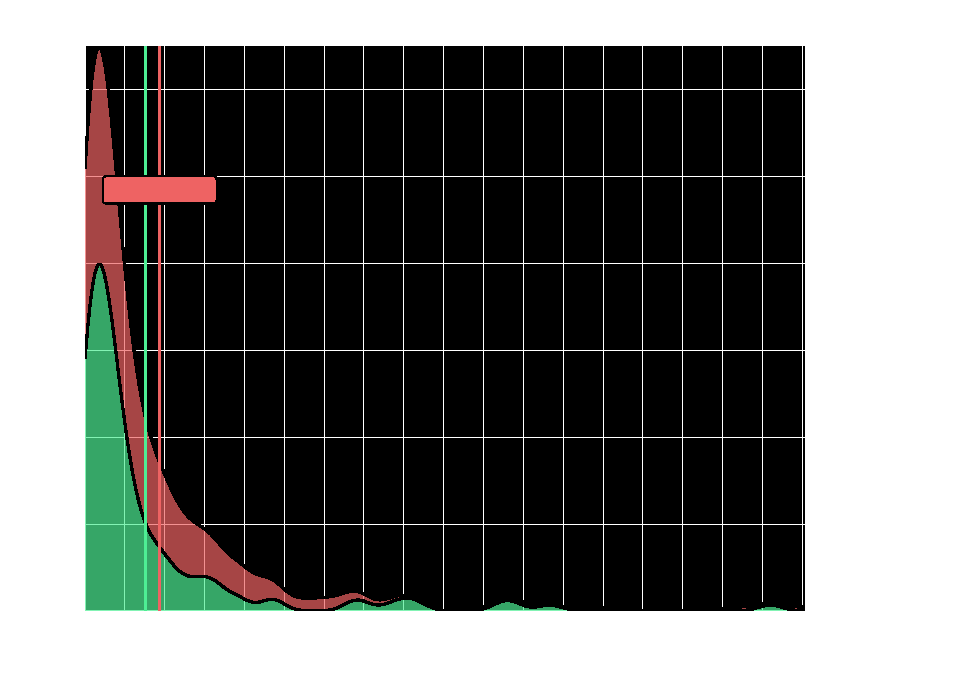
\includegraphics{hw1-lobstrs-eds241_files/figure-latex/unnamed-chunk-8-1.pdf}

\begin{enumerate}
\def\labelenumi{\arabic{enumi})}
\setcounter{enumi}{1}
\tightlist
\item
  grouped by year
\end{enumerate}

\begin{Shaded}
\begin{Highlighting}[]
\NormalTok{jitter\_plot }\OtherTok{\textless{}{-}}\NormalTok{ spiny\_counts }\SpecialCharTok{\%\textgreater{}\%}
  \FunctionTok{ggplot}\NormalTok{(}\FunctionTok{aes}\NormalTok{(}\AttributeTok{x =} \FunctionTok{factor}\NormalTok{(year),  }
             \AttributeTok{y =}\NormalTok{ counts, }
             \AttributeTok{fill =} \FunctionTok{factor}\NormalTok{(year))) }\SpecialCharTok{+}  
  \FunctionTok{geom\_jitter}\NormalTok{(}\AttributeTok{width =} \FloatTok{0.3}\NormalTok{,}
              \AttributeTok{alpha =} \FloatTok{0.5}\NormalTok{,}
              \AttributeTok{shape =} \DecValTok{21}\NormalTok{,}
              \AttributeTok{size =} \DecValTok{3}\NormalTok{,}
              \AttributeTok{show.legend =} \ConstantTok{FALSE}\NormalTok{) }\SpecialCharTok{+}  
  \FunctionTok{stat\_summary}\NormalTok{(}\FunctionTok{aes}\NormalTok{(}\AttributeTok{color =} \StringTok{" "}\NormalTok{),}
               \AttributeTok{fun =} \StringTok{"mean"}\NormalTok{,}
               \AttributeTok{geom =} \StringTok{"crossbar"}\NormalTok{,}
               \AttributeTok{fill =} \StringTok{"white"}\NormalTok{,}
               \AttributeTok{size =} \FloatTok{0.35}\NormalTok{,}
               \AttributeTok{show.legend =} \ConstantTok{TRUE}\NormalTok{) }\SpecialCharTok{+}  
  \FunctionTok{labs}\NormalTok{(}\AttributeTok{title =} \StringTok{"Lobster counts by year"}\NormalTok{,}
       \AttributeTok{x =} \StringTok{"Year"}\NormalTok{, }
       \AttributeTok{y =} \StringTok{"Lobster count"}\NormalTok{,}
       \AttributeTok{color =} \StringTok{"Mean counts"}\NormalTok{) }\SpecialCharTok{+}  
  \FunctionTok{scale\_fill\_viridis\_d}\NormalTok{(}\AttributeTok{guide =} \StringTok{"none"}\NormalTok{) }\SpecialCharTok{+} 
  \FunctionTok{scale\_color\_manual}\NormalTok{(}\AttributeTok{values =} \FunctionTok{c}\NormalTok{(}\StringTok{" "} \OtherTok{=} \StringTok{"black"}\NormalTok{)) }\SpecialCharTok{+}  
  \FunctionTok{scale\_y\_continuous}\NormalTok{(}\AttributeTok{breaks =} \FunctionTok{seq}\NormalTok{(}\DecValTok{0}\NormalTok{,}\DecValTok{300}\NormalTok{,}\DecValTok{25}\NormalTok{)) }\SpecialCharTok{+}
  \FunctionTok{coord\_flip}\NormalTok{() }\SpecialCharTok{+} 
  \FunctionTok{theme\_bw}\NormalTok{() }\SpecialCharTok{+}
  \FunctionTok{theme}\NormalTok{(}\AttributeTok{text =} \FunctionTok{element\_text}\NormalTok{(}\AttributeTok{color =} \StringTok{"white"}\NormalTok{),}
        \AttributeTok{axis.text =} \FunctionTok{element\_text}\NormalTok{(}\AttributeTok{color =} \StringTok{"white"}\NormalTok{),}
        \AttributeTok{legend.text =} \FunctionTok{element\_text}\NormalTok{(}\AttributeTok{color =} \StringTok{"black"}\NormalTok{),}
        \AttributeTok{legend.title =} \FunctionTok{element\_text}\NormalTok{(}\AttributeTok{color =} \StringTok{"black"}\NormalTok{),}
        \AttributeTok{panel.grid =} \FunctionTok{element\_line}\NormalTok{(}\AttributeTok{color =} \StringTok{"black"}\NormalTok{,}
                                  \AttributeTok{linewidth =} \FloatTok{0.1}\NormalTok{),}
        \AttributeTok{panel.background =} \FunctionTok{element\_rect}\NormalTok{(}\AttributeTok{fill =} \StringTok{"white"}\NormalTok{),}
        \AttributeTok{plot.background =} \FunctionTok{element\_rect}\NormalTok{(}\AttributeTok{fill =} \StringTok{"black"}\NormalTok{)) }
\end{Highlighting}
\end{Shaded}

\begin{verbatim}
## Warning: Using `size` aesthetic for lines was deprecated in ggplot2 3.4.0.
## i Please use `linewidth` instead.
## This warning is displayed once every 8 hours.
## Call `lifecycle::last_lifecycle_warnings()` to see where this warning was
## generated.
\end{verbatim}

\begin{Shaded}
\begin{Highlighting}[]
\FunctionTok{print}\NormalTok{(jitter\_plot)}
\end{Highlighting}
\end{Shaded}

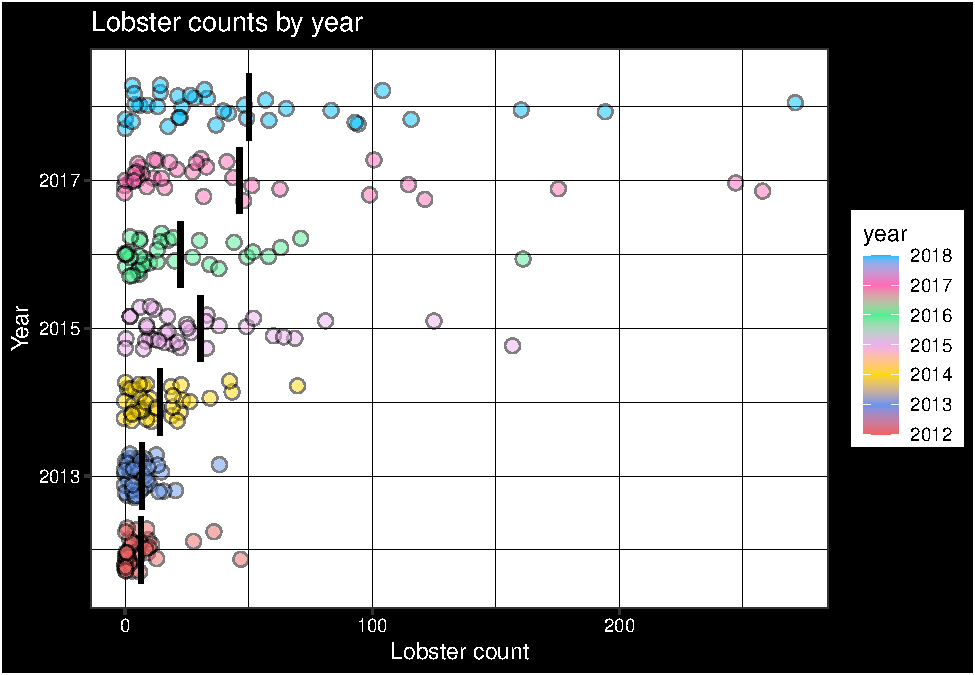
\includegraphics{hw1-lobstrs-eds241_files/figure-latex/unnamed-chunk-9-1.pdf}

\begin{enumerate}
\def\labelenumi{\arabic{enumi})}
\setcounter{enumi}{2}
\tightlist
\item
  grouped by site
\end{enumerate}

\begin{Shaded}
\begin{Highlighting}[]
\NormalTok{violin\_plot }\OtherTok{\textless{}{-}}\NormalTok{ spiny\_counts }\SpecialCharTok{\%\textgreater{}\%}
  \FunctionTok{ggplot}\NormalTok{(}\FunctionTok{aes}\NormalTok{(}\AttributeTok{x =}\NormalTok{ site, }\AttributeTok{y =}\NormalTok{ counts, }
             \AttributeTok{fill =}\NormalTok{ site)) }\SpecialCharTok{+}
  \FunctionTok{geom\_violin}\NormalTok{(}\AttributeTok{alpha =} \FloatTok{0.9}\NormalTok{,}
              \AttributeTok{width =} \FloatTok{1.2}\NormalTok{) }\SpecialCharTok{+}  
  \FunctionTok{theme\_bw}\NormalTok{() }\SpecialCharTok{+}
  \FunctionTok{theme}\NormalTok{(}\AttributeTok{text =} \FunctionTok{element\_text}\NormalTok{(}\AttributeTok{color =} \StringTok{"white"}\NormalTok{),}
        \AttributeTok{axis.text =} \FunctionTok{element\_text}\NormalTok{(}\AttributeTok{color =} \StringTok{"white"}\NormalTok{),}
        \AttributeTok{legend.text =} \FunctionTok{element\_text}\NormalTok{(}\AttributeTok{color =} \StringTok{"black"}\NormalTok{),}
        \AttributeTok{legend.title =} \FunctionTok{element\_text}\NormalTok{(}\AttributeTok{color =} \StringTok{"black"}\NormalTok{),}
        \AttributeTok{panel.grid =} \FunctionTok{element\_line}\NormalTok{(}\AttributeTok{color =} \StringTok{"black"}\NormalTok{,}
                                  \AttributeTok{linewidth =} \FloatTok{0.1}\NormalTok{),}
        \AttributeTok{panel.background =} \FunctionTok{element\_rect}\NormalTok{(}\AttributeTok{fill =} \StringTok{"white"}\NormalTok{),}
        \AttributeTok{plot.background =} \FunctionTok{element\_rect}\NormalTok{(}\AttributeTok{fill =} \StringTok{"black"}\NormalTok{)) }\SpecialCharTok{+}
  \FunctionTok{labs}\NormalTok{(}\AttributeTok{title =} \StringTok{"Lobster counts by reef site"}\NormalTok{,}
       \AttributeTok{fill =} \StringTok{"Site"}\NormalTok{,}
       \AttributeTok{x =} \StringTok{"Site"}\NormalTok{, }
       \AttributeTok{y =} \StringTok{"Lobster count"}\NormalTok{) }\SpecialCharTok{+}
  \FunctionTok{stat\_summary}\NormalTok{(}
    \FunctionTok{aes}\NormalTok{(}\AttributeTok{label =} \FunctionTok{paste0}\NormalTok{(}\StringTok{"Mdn "}\NormalTok{,}\StringTok{""}\NormalTok{,}\FunctionTok{round}\NormalTok{(..y.., }\DecValTok{1}\NormalTok{))),}
    \AttributeTok{size =} \DecValTok{2}\NormalTok{,}
    \AttributeTok{fun =} \StringTok{"median"}\NormalTok{,}
    \AttributeTok{geom =} \StringTok{"text"}\NormalTok{,}
    \AttributeTok{colour =} \StringTok{"black"}\NormalTok{,}
    \AttributeTok{show.legend =} \ConstantTok{FALSE}\NormalTok{) }\SpecialCharTok{+}
  \FunctionTok{scale\_fill\_manual}\NormalTok{(}\AttributeTok{values =} \FunctionTok{c}\NormalTok{(}
    \StringTok{"indianred2"}\NormalTok{, }\StringTok{"cornflowerblue"}\NormalTok{, }\StringTok{"gold1"}\NormalTok{, }\StringTok{"plum2"}\NormalTok{, }\StringTok{"seagreen2"}
\NormalTok{  )) }\SpecialCharTok{+}
  \FunctionTok{scale\_color\_manual}\NormalTok{(}\AttributeTok{values =} \FunctionTok{c}\NormalTok{(}
    \StringTok{"indianred2"}\NormalTok{, }\StringTok{"cornflowerblue"}\NormalTok{, }\StringTok{"gold1"}\NormalTok{, }\StringTok{"plum2"}\NormalTok{, }\StringTok{"seagreen2"}\NormalTok{))}\SpecialCharTok{+}
  \FunctionTok{scale\_y\_continuous}\NormalTok{(}\AttributeTok{breaks =} \FunctionTok{seq}\NormalTok{(}\DecValTok{0}\NormalTok{,}\DecValTok{300}\NormalTok{,}\DecValTok{25}\NormalTok{)) }\SpecialCharTok{+}
  \FunctionTok{coord\_flip}\NormalTok{() }
  

\FunctionTok{print}\NormalTok{(violin\_plot)}
\end{Highlighting}
\end{Shaded}

\begin{verbatim}
## Warning: The dot-dot notation (`..y..`) was deprecated in ggplot2 3.4.0.
## i Please use `after_stat(y)` instead.
## This warning is displayed once every 8 hours.
## Call `lifecycle::last_lifecycle_warnings()` to see where this warning was
## generated.
\end{verbatim}

\begin{verbatim}
## Warning: `position_dodge()` requires non-overlapping x intervals.
\end{verbatim}

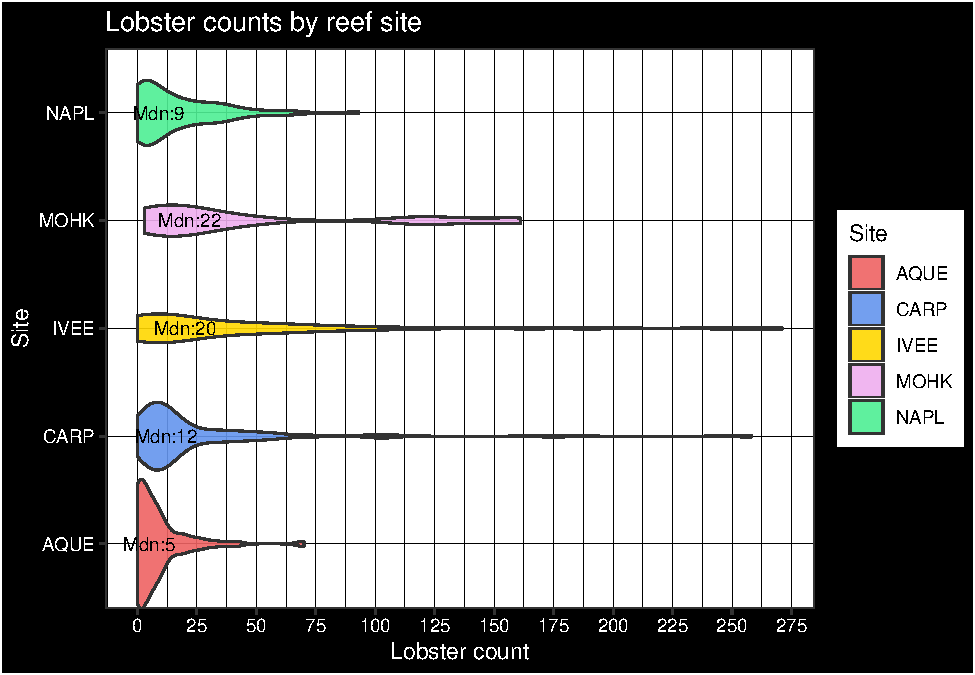
\includegraphics{hw1-lobstrs-eds241_files/figure-latex/unnamed-chunk-10-1.pdf}

Create a plot of lobster \textbf{size} :

\begin{enumerate}
\def\labelenumi{\arabic{enumi})}
\setcounter{enumi}{3}
\tightlist
\item
  You choose the grouping variable(s)!
\end{enumerate}

\begin{Shaded}
\begin{Highlighting}[]
\NormalTok{medians }\OtherTok{\textless{}{-}}\NormalTok{ spiny\_counts }\SpecialCharTok{\%\textgreater{}\%}
  \FunctionTok{group\_by}\NormalTok{(site) }\SpecialCharTok{\%\textgreater{}\%}
  \FunctionTok{summarize}\NormalTok{(}\AttributeTok{median\_size =} \FunctionTok{median}\NormalTok{(mean\_size, }\AttributeTok{na.rm =} \ConstantTok{TRUE}\NormalTok{))}

\NormalTok{spiny\_counts }\SpecialCharTok{\%\textgreater{}\%} 
  \FunctionTok{ggplot}\NormalTok{(}\FunctionTok{aes}\NormalTok{(}\AttributeTok{x =}\NormalTok{ mean\_size, }\AttributeTok{y =}\NormalTok{ site, }\AttributeTok{fill =}\NormalTok{ site)) }\SpecialCharTok{+}
  \FunctionTok{geom\_density\_ridges}\NormalTok{(}
    \AttributeTok{alpha =} \FloatTok{0.5}\NormalTok{,}
    \AttributeTok{size =} \DecValTok{1}\NormalTok{,}
    \AttributeTok{scale =} \DecValTok{2}
\NormalTok{  ) }\SpecialCharTok{+}
  \FunctionTok{geom\_text}\NormalTok{(}\AttributeTok{data =}\NormalTok{ medians, }
            \FunctionTok{aes}\NormalTok{(}\AttributeTok{x =}\NormalTok{ median\_size, }
                \AttributeTok{y =}\NormalTok{ site, }
                \AttributeTok{label =} \FunctionTok{paste0}\NormalTok{(}\StringTok{"Median"}\NormalTok{,}\StringTok{" "}\NormalTok{,(}\FunctionTok{round}\NormalTok{(median\_size, }\DecValTok{2}\NormalTok{)))),}
            \AttributeTok{color =} \StringTok{"black"}\NormalTok{, }
            \AttributeTok{size =} \DecValTok{2}\NormalTok{, }
            \AttributeTok{vjust =} \SpecialCharTok{{-}}\FloatTok{0.75}\NormalTok{) }\SpecialCharTok{+}
  \FunctionTok{theme}\NormalTok{(}\AttributeTok{text =} \FunctionTok{element\_text}\NormalTok{(}\AttributeTok{color =} \StringTok{"white"}\NormalTok{),}
        \AttributeTok{axis.text =} \FunctionTok{element\_text}\NormalTok{(}\AttributeTok{color =} \StringTok{"white"}\NormalTok{),}
        \AttributeTok{legend.position =} \StringTok{"none"}\NormalTok{,}
        \AttributeTok{panel.grid =} \FunctionTok{element\_line}\NormalTok{(}\AttributeTok{color =} \StringTok{"black"}\NormalTok{,}
                                  \AttributeTok{linewidth =} \FloatTok{0.1}\NormalTok{),}
        \AttributeTok{panel.background =} \FunctionTok{element\_rect}\NormalTok{(}\AttributeTok{fill =} \StringTok{"white"}\NormalTok{),}
        \AttributeTok{plot.background =} \FunctionTok{element\_rect}\NormalTok{(}\AttributeTok{fill =} \StringTok{"black"}\NormalTok{)) }\SpecialCharTok{+}
  \FunctionTok{labs}\NormalTok{(}
    \AttributeTok{title =} \StringTok{"Density of lobster mean size by reef site"}\NormalTok{,}
    \AttributeTok{x =} \StringTok{"Lobster mean size"}\NormalTok{, }
    \AttributeTok{y =} \StringTok{"Reef site"}\NormalTok{,}
    \AttributeTok{fill =} \StringTok{"Site"}
\NormalTok{  ) }\SpecialCharTok{+} 
  \FunctionTok{scale\_fill\_manual}\NormalTok{(}\AttributeTok{values =} \FunctionTok{c}\NormalTok{(}
    \StringTok{"indianred2"}\NormalTok{, }\StringTok{"cornflowerblue"}\NormalTok{, }\StringTok{"gold1"}\NormalTok{, }\StringTok{"plum2"}\NormalTok{, }\StringTok{"seagreen2"}
\NormalTok{  )) }
\end{Highlighting}
\end{Shaded}

\begin{verbatim}
## Warning in geom_density_ridges(alpha = 0.5, size = 1, scale = 2): Ignoring
## unknown parameters: `size`
\end{verbatim}

\begin{verbatim}
## Picking joint bandwidth of 2.32
\end{verbatim}

\begin{verbatim}
## Warning: Removed 27 rows containing non-finite outside the scale range
## (`stat_density_ridges()`).
\end{verbatim}

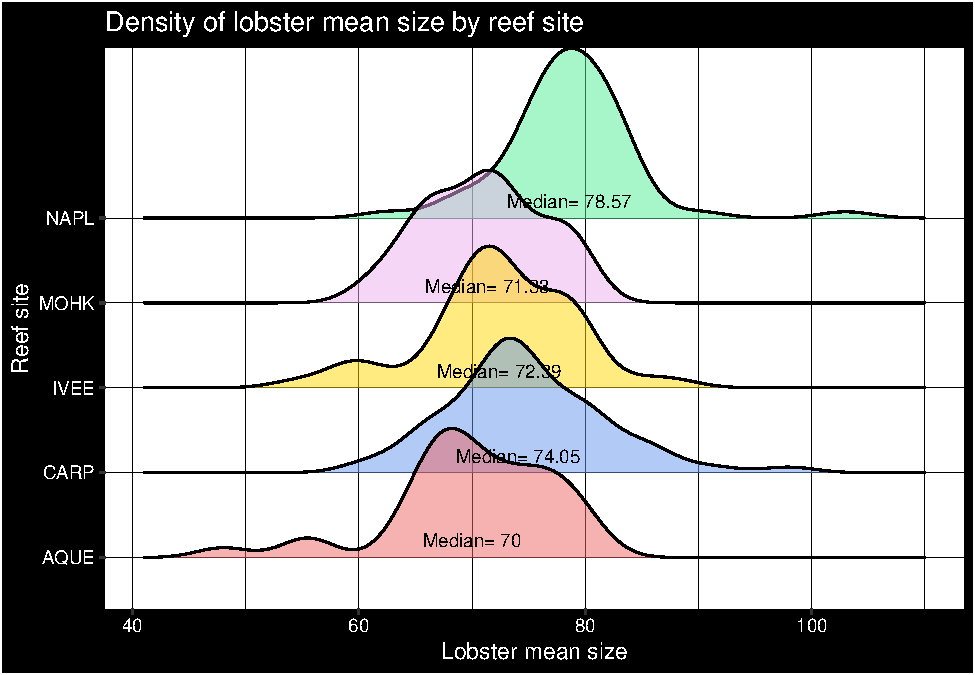
\includegraphics{hw1-lobstrs-eds241_files/figure-latex/unnamed-chunk-11-1.pdf}

\textbf{c.} Compare means of the outcome by treatment group. Using the
\texttt{tbl\_summary()} function from the package
\href{https://www.danieldsjoberg.com/gtsummary/articles/tbl_summary.html}{\texttt{gt\_summary}}

\begin{Shaded}
\begin{Highlighting}[]
\NormalTok{spiny\_counts }\SpecialCharTok{\%\textgreater{}\%}
  \FunctionTok{ungroup}\NormalTok{() }\SpecialCharTok{\%\textgreater{}\%}
  \FunctionTok{tbl\_summary}\NormalTok{(.,}
            \AttributeTok{by =} \StringTok{"mpa"}\NormalTok{,}
            \AttributeTok{statistic =} \FunctionTok{list}\NormalTok{(}\FunctionTok{all\_continuous}\NormalTok{() }\SpecialCharTok{\textasciitilde{}} \StringTok{"\{mean\}"}\NormalTok{),}
            \AttributeTok{include =} \StringTok{"site"}\NormalTok{) }
\end{Highlighting}
\end{Shaded}

\begin{table}[!t]
\fontsize{12.0pt}{14.4pt}\selectfont
\begin{tabular*}{\linewidth}{@{\extracolsep{\fill}}lcc}
\toprule
\textbf{Characteristic} & \textbf{MPA}  N = 119\textsuperscript{\textit{1}} & \textbf{non\_MPA}  N = 133\textsuperscript{\textit{1}} \\ 
\midrule\addlinespace[2.5pt]
site &  &  \\ 
    AQUE & 0 (0\%) & 49 (37\%) \\ 
    CARP & 0 (0\%) & 63 (47\%) \\ 
    IVEE & 56 (47\%) & 0 (0\%) \\ 
    MOHK & 0 (0\%) & 21 (16\%) \\ 
    NAPL & 63 (53\%) & 0 (0\%) \\ 
\bottomrule
\end{tabular*}
\begin{minipage}{\linewidth}
\textsuperscript{\textit{1}}n (\%)\\
\end{minipage}
\end{table}

\begin{center}\rule{0.5\linewidth}{0.5pt}\end{center}

Step 4: OLS regression- building intuition

\textbf{a.} Start with a simple OLS estimator of lobster counts
regressed on treatment. Use the function \texttt{summ()} from the
\href{https://jtools.jacob-long.com/}{\texttt{jtools}} package to print
the OLS output

\begin{Shaded}
\begin{Highlighting}[]
\CommentTok{\# }\AlertTok{NOTE}\CommentTok{: We will not evaluate/interpret model fit in this assignment (e.g., R{-}square)}

\NormalTok{m1\_ols }\OtherTok{\textless{}{-}} \FunctionTok{lm}\NormalTok{(counts }\SpecialCharTok{\textasciitilde{}}\NormalTok{ treat,}
             \AttributeTok{data =}\NormalTok{ spiny\_counts) }

\NormalTok{tbl\_1 }\OtherTok{\textless{}{-}} \FunctionTok{summ}\NormalTok{(}\AttributeTok{model =}\NormalTok{ m1\_ols,}
     \AttributeTok{model.fit =} \ConstantTok{FALSE}\NormalTok{) }

\FunctionTok{print}\NormalTok{(tbl\_1)}
\end{Highlighting}
\end{Shaded}

\begin{verbatim}
## MODEL INFO:
## Observations: 252
## Dependent Variable: counts
## Type: OLS linear regression 
## 
## Standard errors:OLS
## ------------------------------------------------
##                      Est.   S.E.   t val.      p
## ----------------- ------- ------ -------- ------
## (Intercept)         22.73   3.57     6.36   0.00
## treat                5.36   5.20     1.03   0.30
## ------------------------------------------------
\end{verbatim}

\textbf{b.} Interpret the intercept \& predictor coefficients \emph{in
your own words}. Use full sentences and write your interpretation of the
regression results to be as clear as possible to a non-academic
audience.

The intercept = 22.73 is what the lm model estimates the average lobster
count will be when the treatment is not being applied (when the site is
not an MPA site). The predictor coeffient = 5.36 tells us that when the
treatment IS applied (the site is an MPA) the estimated average lobster
count will increase from 22.73 by 5.36. The predictor tells us that
sites that are MPAs have a positive effect on lobster counts (lobsters
are more abundant), in average, since the model is estimating across all
the observations.

\textbf{c.} Check the model assumptions using the \texttt{check\_model}
function from the \texttt{performance} package

\textbf{d.} Explain the results of the 4 diagnostic plots. Why are we
getting this result?

\begin{Shaded}
\begin{Highlighting}[]
\FunctionTok{check\_model}\NormalTok{(m1\_ols, }\AttributeTok{check =} \StringTok{"qq"}\NormalTok{ )}
\end{Highlighting}
\end{Shaded}

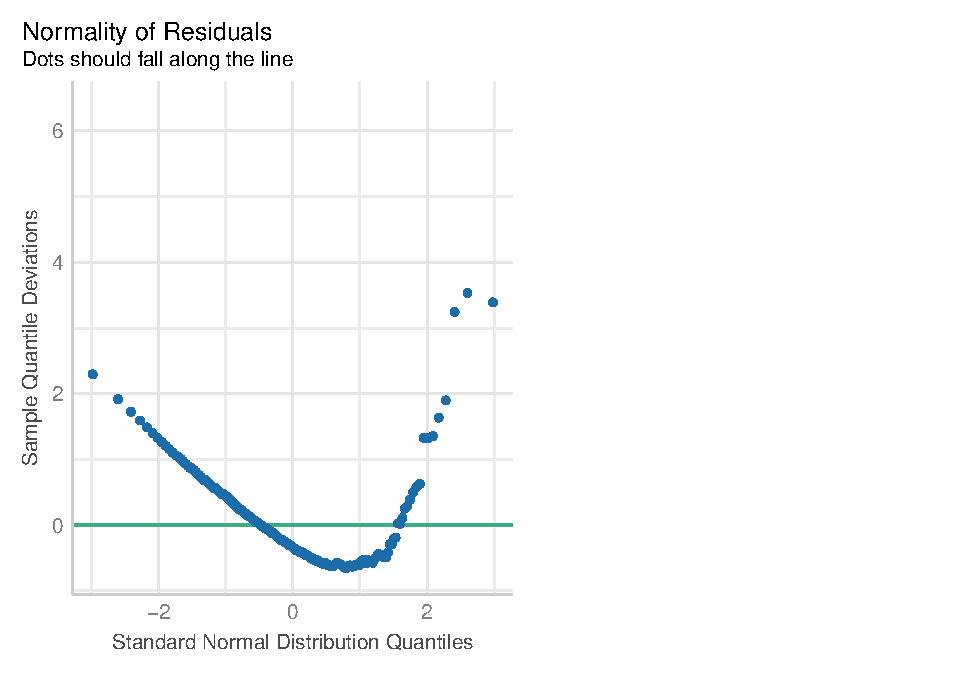
\includegraphics{hw1-lobstrs-eds241_files/figure-latex/unnamed-chunk-14-1.pdf}
\textbf{QQ plot explanation} The straight line represents a normal
distribution and the model's residuals diverge significantly from it.
There is a noticeable pattern in our residuals when the distribution of
normal residuals should have no pattern/be randomly distributed. This
tells us we are more than likely using the wrong model for our data and
we are not capturing the effect of possible patterns in it.

\begin{Shaded}
\begin{Highlighting}[]
\FunctionTok{check\_model}\NormalTok{(m1\_ols, }\AttributeTok{check =} \StringTok{"normality"}\NormalTok{)}
\end{Highlighting}
\end{Shaded}

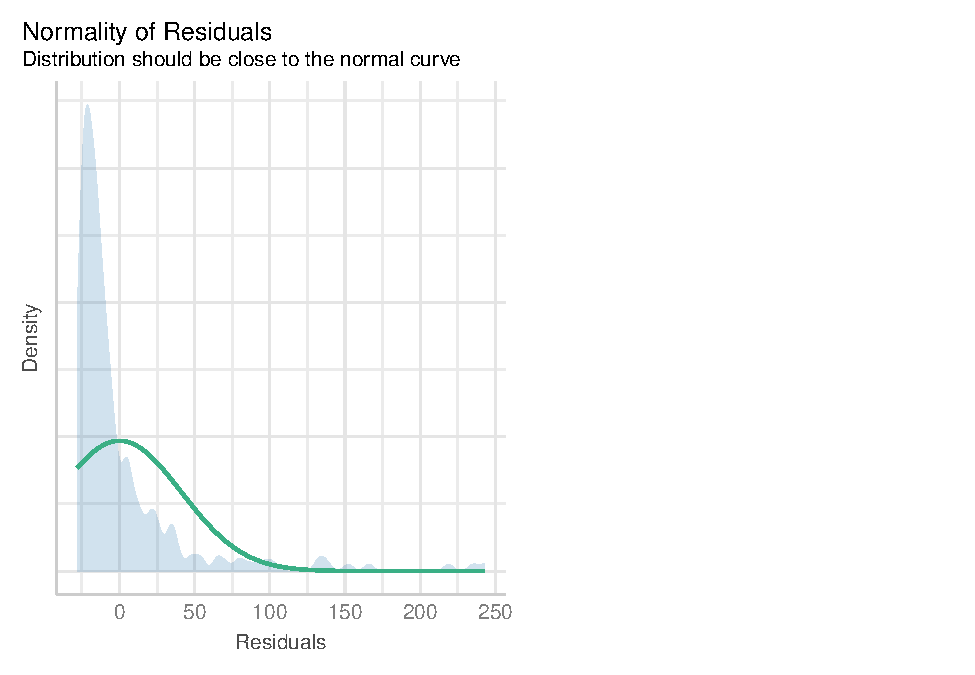
\includegraphics{hw1-lobstrs-eds241_files/figure-latex/unnamed-chunk-15-1.pdf}
\textbf{Normality of residuals density plot explanation} Plot indicates
a departure from normality and it allows us to see HOW our model
predictions deviate from a normal distribution. Our data is likely
skewed (not symmetrically distributed) and has a tail.

\begin{Shaded}
\begin{Highlighting}[]
\FunctionTok{check\_model}\NormalTok{(m1\_ols, }\AttributeTok{check =} \StringTok{"homogeneity"}\NormalTok{)}
\end{Highlighting}
\end{Shaded}

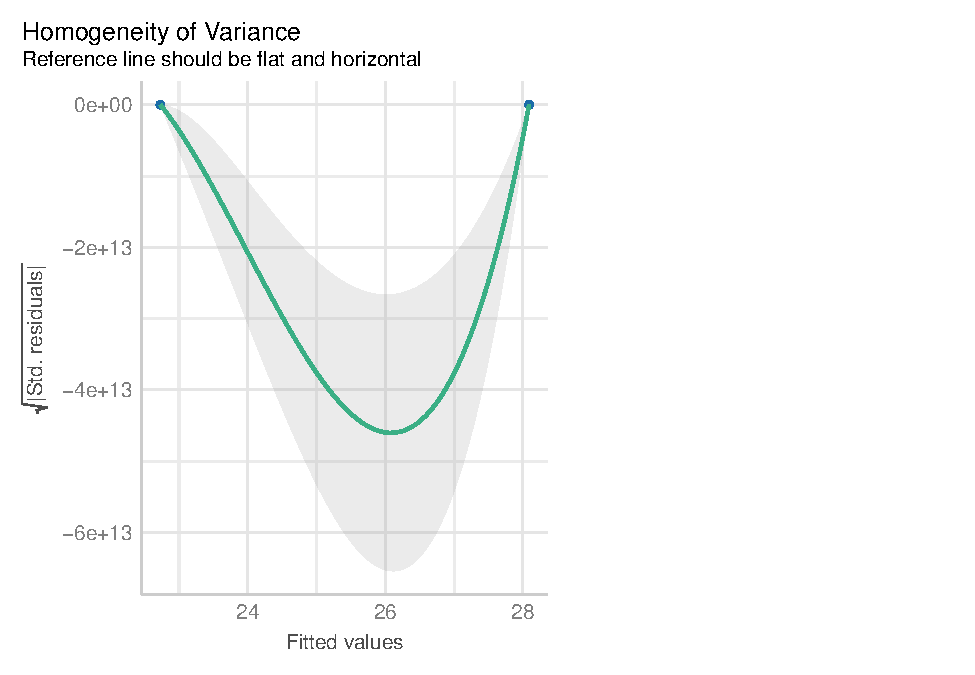
\includegraphics{hw1-lobstrs-eds241_files/figure-latex/unnamed-chunk-16-1.pdf}
\textbf{Homogeneity of variance plot explanation} This plot shows that
the residuals of our fitted values do not display constant variance
across all levels, this means that the model does not accurately capture
the variability of all levels in our data.

\begin{Shaded}
\begin{Highlighting}[]
\FunctionTok{check\_model}\NormalTok{(m1\_ols, }\AttributeTok{check =} \StringTok{"pp\_check"}\NormalTok{)}
\end{Highlighting}
\end{Shaded}

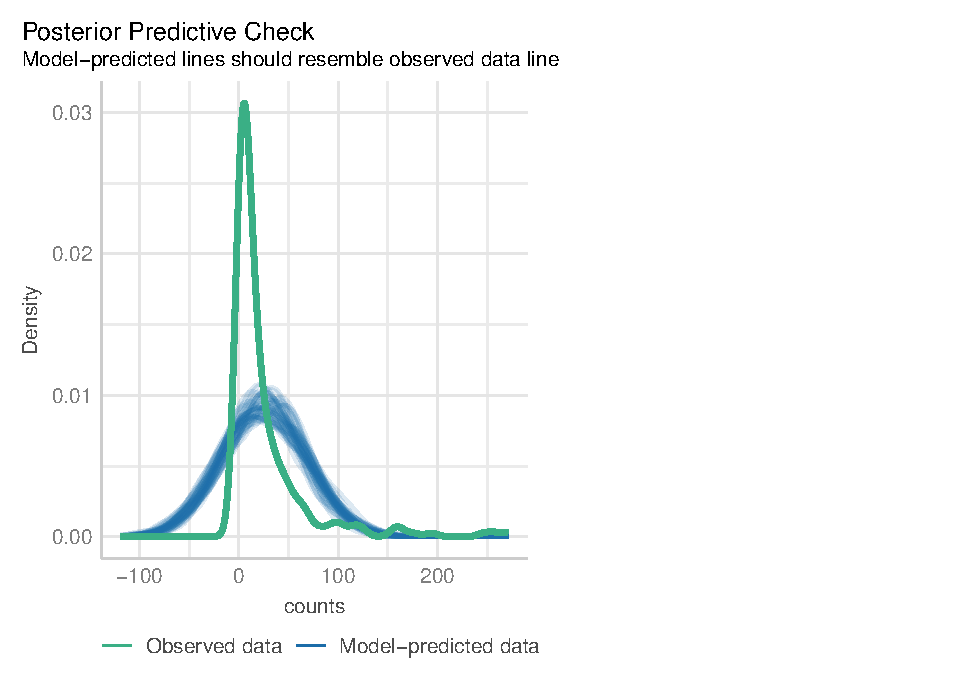
\includegraphics{hw1-lobstrs-eds241_files/figure-latex/unnamed-chunk-17-1.pdf}
\textbf{Posterior predictive check explanation} This plot tells us that
the distribution of our model data predictions do not match those that
were actually observed. It speaks to a poor model fit. The model does
not seem to be accurately representing and replicating the complexity of
the observed data.
------------------------------------------------------------------------

Step 5: Fitting GLMs

\textbf{a.} Estimate a Poisson regression model using the \texttt{glm()}
function

\begin{Shaded}
\begin{Highlighting}[]
\NormalTok{m2\_pois }\OtherTok{\textless{}{-}} \FunctionTok{glm}\NormalTok{(counts }\SpecialCharTok{\textasciitilde{}}\NormalTok{ treat, }
                   \AttributeTok{data =}\NormalTok{ spiny\_counts,}
                   \AttributeTok{family =} \FunctionTok{poisson}\NormalTok{(}\AttributeTok{link =} \StringTok{"log"}\NormalTok{)) }

\FunctionTok{exp}\NormalTok{(}\FunctionTok{coef}\NormalTok{(m2\_pois))}
\end{Highlighting}
\end{Shaded}

\begin{verbatim}
## (Intercept)       treat 
##   22.729323    1.235956
\end{verbatim}

\begin{Shaded}
\begin{Highlighting}[]
\FunctionTok{summary}\NormalTok{(m2\_pois)}
\end{Highlighting}
\end{Shaded}

\begin{verbatim}
## 
## Call:
## glm(formula = counts ~ treat, family = poisson(link = "log"), 
##     data = spiny_counts)
## 
## Coefficients:
##             Estimate Std. Error z value Pr(>|z|)    
## (Intercept)  3.12366    0.01819 171.744   <2e-16 ***
## treat        0.21184    0.02510   8.441   <2e-16 ***
## ---
## Signif. codes:  0 '***' 0.001 '**' 0.01 '*' 0.05 '.' 0.1 ' ' 1
## 
## (Dispersion parameter for poisson family taken to be 1)
## 
##     Null deviance: 10438  on 251  degrees of freedom
## Residual deviance: 10366  on 250  degrees of freedom
## AIC: 11366
## 
## Number of Fisher Scoring iterations: 6
\end{verbatim}

\textbf{b.} Interpret the predictor coefficient in your own words. Use
full sentences and write your interpretation of the results to be as
clear as possible to a non-academic audience.

The model estimates how the treatment affects the lobster count of any
given site. Meaning, in a reef site that is not an MPA the lobster count
is estimated to be aprox. 23. When the treatment is applied (when the
reef site is an MPA), model estimates a multiplicative factor of approx.
1.24. This means the model predicts an increase in lobster count when
the treatment is applied (when the reef is an MPA)

\textbf{c.} Explain the statistical concept of dispersion and
overdispersion in the context of this model.

Dispersion is the spread/distribution of variability around the mean. A
poisson model makes the assumption that the mean and variance of the
data are equal to each other. Overdispersion in this case would mean
that the variability predicted by the model is greater than the mean of
the data. This means that the model may not be a good fit - it may not
account for all the variability occurring in the data. There may be
other interactions at play across sites and lobster counts that are
unaccounted for.

\textbf{d.} Compare results with previous model, explain change in the
significance of the treatment effect

The previous model (OLS) gave us a 5.36 coefficient for the treatment
varible, but its p-value was 0.30, which is not statistically
significant. Unlike the OLS model, the glm model gave us (when
exponentiated) the percent change for one unit increase in the predictor
and its p-value was highly significant. The change in the significance
of the treatment effect is a result of the original OLS model being a
poor fit for our data since we have counts data and overdispersion is
present. OLS makes the assumption that our residuals are normally
distributed and our data non-discrete, which is not the case here.

\begin{Shaded}
\begin{Highlighting}[]
\CommentTok{\#HINT1: Incidence Ratio Rate (IRR): Exponentiation of beta returns coefficient which is interpreted as the \textquotesingle{}percent change\textquotesingle{} for a one unit increase in the predictor }

\CommentTok{\#HINT2: For the second glm() argument \textasciigrave{}family\textasciigrave{} use the following specification option \textasciigrave{}family = poisson(link = "log")\textasciigrave{}}
\CommentTok{\#}
\NormalTok{m2\_pois }\OtherTok{\textless{}{-}} \FunctionTok{glm}\NormalTok{(counts }\SpecialCharTok{\textasciitilde{}}\NormalTok{ treat, }
                   \AttributeTok{data =}\NormalTok{ spiny\_counts,}
                   \AttributeTok{family =} \FunctionTok{poisson}\NormalTok{(}\AttributeTok{link =} \StringTok{"log"}\NormalTok{)) }
\end{Highlighting}
\end{Shaded}

\textbf{e.} Check the model assumptions. Explain results.

The posterior predictive check uses data simulated from the model and
compares it to the actual observed data. The PPC plot shows a
discrepancy between the simulated and the observed outcomes. What the
model is predicting is not what is being observed, pointing to a poor
model fit. The residual variance as predicted by the model also does not
align with the observed, another sign that the model is not capturing
the true mechanisms at work within the data. There is no homogeneity in
the variance of the observed when compared to the predicted, indicating
that model does not capture the differences in variance across our data,
it assumes homogeneity.

\textbf{f.} Conduct tests for over-dispersion \& zero-inflation. Explain
results.

\begin{Shaded}
\begin{Highlighting}[]
\FunctionTok{check\_model}\NormalTok{(m2\_pois)}
\end{Highlighting}
\end{Shaded}

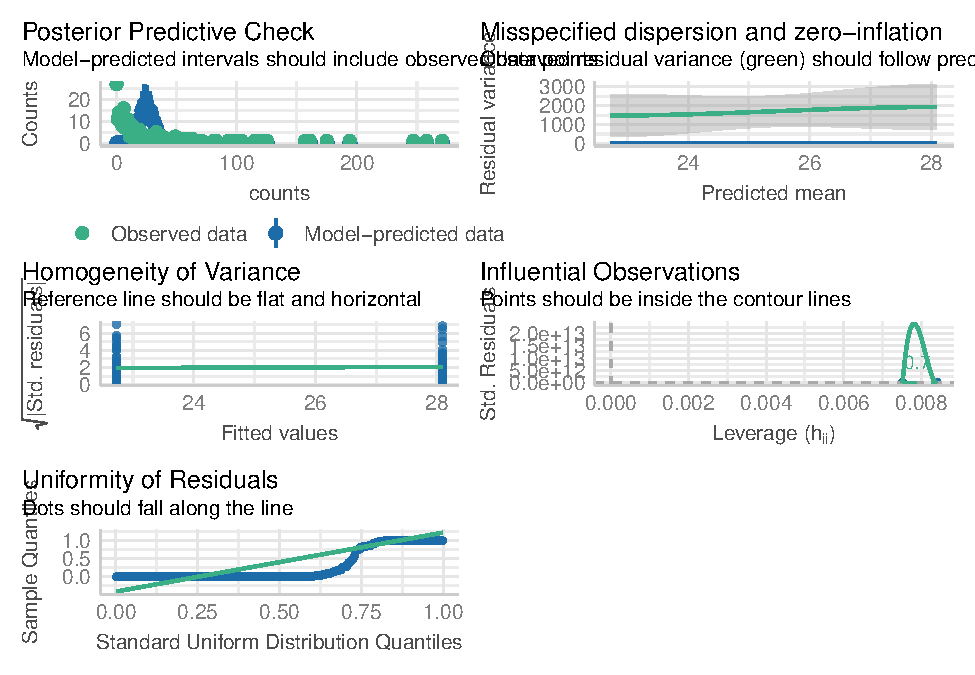
\includegraphics{hw1-lobstrs-eds241_files/figure-latex/unnamed-chunk-20-1.pdf}

\begin{Shaded}
\begin{Highlighting}[]
\FunctionTok{check\_overdispersion}\NormalTok{(m2\_pois)}
\end{Highlighting}
\end{Shaded}

\begin{verbatim}
## # Overdispersion test
## 
##        dispersion ratio =    67.033
##   Pearson's Chi-Squared = 16758.289
##                 p-value =   < 0.001
\end{verbatim}

\begin{verbatim}
## Overdispersion detected.
\end{verbatim}

\textbf{Overdispersion test explanation} The test shows a dispersion
ratio of 67.033. A dispersion \textgreater{} 1 is considered
overdispersion. The p-value of our test is very small, certainly
significant. This means that we can confidently say there is more
variability in the data than the model can predict.

\begin{Shaded}
\begin{Highlighting}[]
\FunctionTok{check\_zeroinflation}\NormalTok{(m2\_pois)}
\end{Highlighting}
\end{Shaded}

\begin{verbatim}
## # Check for zero-inflation
## 
##    Observed zeros: 27
##   Predicted zeros: 0
##             Ratio: 0.00
\end{verbatim}

\begin{verbatim}
## Model is underfitting zeros (probable zero-inflation).
\end{verbatim}

\textbf{Zero-inflation explanation} The results of the test say that the
model did not predict/account for ANY zeros being present in our data.
However, our data did contain 27 observations that were = 0. This means
that the model is underfitting our data and our data is inflated - it
contains more zero values than the model accounts for.

\textbf{g.} Fit a negative binomial model using the function glm.nb()
from the package \texttt{MASS} and check model diagnostics

\begin{Shaded}
\begin{Highlighting}[]
\NormalTok{m3\_nb }\OtherTok{\textless{}{-}} \FunctionTok{glm.nb}\NormalTok{(counts }\SpecialCharTok{\textasciitilde{}}\NormalTok{ treat,}
                \AttributeTok{data =}\NormalTok{ spiny\_counts)}

\FunctionTok{summary}\NormalTok{(m3\_nb)}
\end{Highlighting}
\end{Shaded}

\begin{verbatim}
## 
## Call:
## glm.nb(formula = counts ~ treat, data = spiny_counts, init.theta = 0.5500333101, 
##     link = log)
## 
## Coefficients:
##             Estimate Std. Error z value Pr(>|z|)    
## (Intercept)   3.1237     0.1183  26.399   <2e-16 ***
## treat         0.2118     0.1720   1.232    0.218    
## ---
## Signif. codes:  0 '***' 0.001 '**' 0.01 '*' 0.05 '.' 0.1 ' ' 1
## 
## (Dispersion parameter for Negative Binomial(0.55) family taken to be 1)
## 
##     Null deviance: 302.18  on 251  degrees of freedom
## Residual deviance: 300.66  on 250  degrees of freedom
## AIC: 2088.5
## 
## Number of Fisher Scoring iterations: 1
## 
## 
##               Theta:  0.5500 
##           Std. Err.:  0.0466 
## 
##  2 x log-likelihood:  -2082.5280
\end{verbatim}

\textbf{h.} In 1-2 sentences explain rationale for fitting this GLM
model.

A negative binomial model allows for overdispersion, whereas a regular
glm poission model does not. Since we tested for dispersion and found a
significantly large dispersion ratio, we need to fit a model that can
accommodate for this overdispersion.

\textbf{i.} Interpret the treatment estimate result in your own words.
Compare with results from the previous model.

\begin{Shaded}
\begin{Highlighting}[]
\CommentTok{\# }\AlertTok{NOTE}\CommentTok{: The \textasciigrave{}glm.nb()\textasciigrave{} function does not require a \textasciigrave{}family\textasciigrave{} argument}

\NormalTok{m3\_nb }\OtherTok{\textless{}{-}} \FunctionTok{glm.nb}\NormalTok{(counts }\SpecialCharTok{\textasciitilde{}}\NormalTok{ treat,}
                \AttributeTok{data =}\NormalTok{ spiny\_counts)}

\FunctionTok{summary}\NormalTok{(m3\_nb)}
\end{Highlighting}
\end{Shaded}

\begin{verbatim}
## 
## Call:
## glm.nb(formula = counts ~ treat, data = spiny_counts, init.theta = 0.5500333101, 
##     link = log)
## 
## Coefficients:
##             Estimate Std. Error z value Pr(>|z|)    
## (Intercept)   3.1237     0.1183  26.399   <2e-16 ***
## treat         0.2118     0.1720   1.232    0.218    
## ---
## Signif. codes:  0 '***' 0.001 '**' 0.01 '*' 0.05 '.' 0.1 ' ' 1
## 
## (Dispersion parameter for Negative Binomial(0.55) family taken to be 1)
## 
##     Null deviance: 302.18  on 251  degrees of freedom
## Residual deviance: 300.66  on 250  degrees of freedom
## AIC: 2088.5
## 
## Number of Fisher Scoring iterations: 1
## 
## 
##               Theta:  0.5500 
##           Std. Err.:  0.0466 
## 
##  2 x log-likelihood:  -2082.5280
\end{verbatim}

\begin{Shaded}
\begin{Highlighting}[]
\FunctionTok{check\_overdispersion}\NormalTok{(m3\_nb)}
\end{Highlighting}
\end{Shaded}

\begin{verbatim}
## # Overdispersion test
## 
##  dispersion ratio = 1.398
##           p-value = 0.088
\end{verbatim}

\begin{verbatim}
## No overdispersion detected.
\end{verbatim}

\begin{Shaded}
\begin{Highlighting}[]
\FunctionTok{check\_zeroinflation}\NormalTok{(m3\_nb)}
\end{Highlighting}
\end{Shaded}

\begin{verbatim}
## # Check for zero-inflation
## 
##    Observed zeros: 27
##   Predicted zeros: 30
##             Ratio: 1.12
\end{verbatim}

\begin{verbatim}
## Model is overfitting zeros (p = 0.600).
\end{verbatim}

\begin{Shaded}
\begin{Highlighting}[]
\FunctionTok{check\_predictions}\NormalTok{(m3\_nb)}
\end{Highlighting}
\end{Shaded}

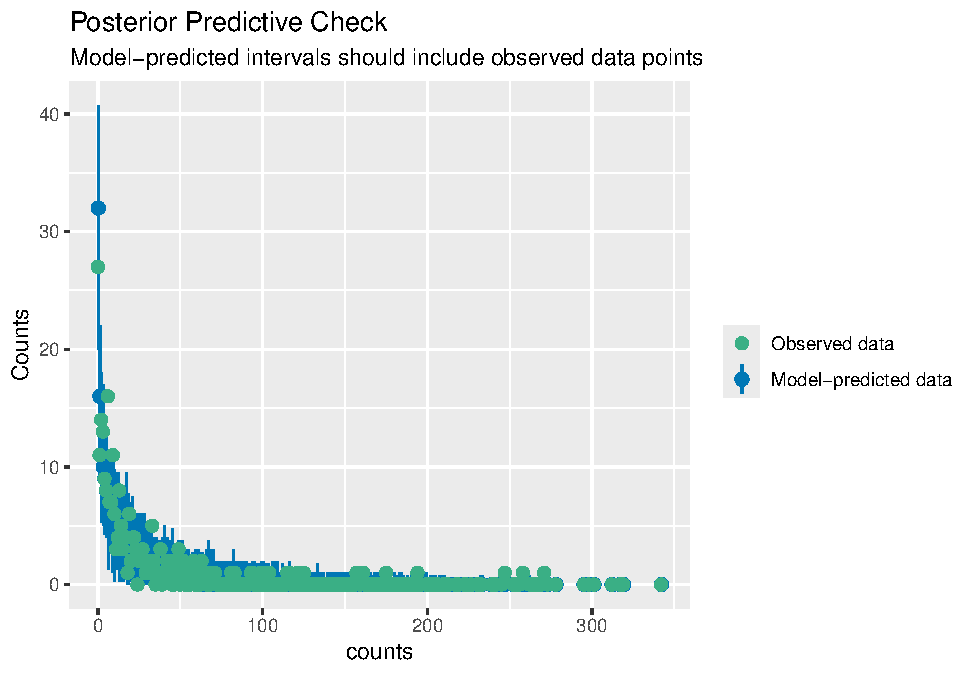
\includegraphics{hw1-lobstrs-eds241_files/figure-latex/unnamed-chunk-27-1.pdf}

\begin{Shaded}
\begin{Highlighting}[]
\FunctionTok{check\_model}\NormalTok{(m3\_nb)}
\end{Highlighting}
\end{Shaded}

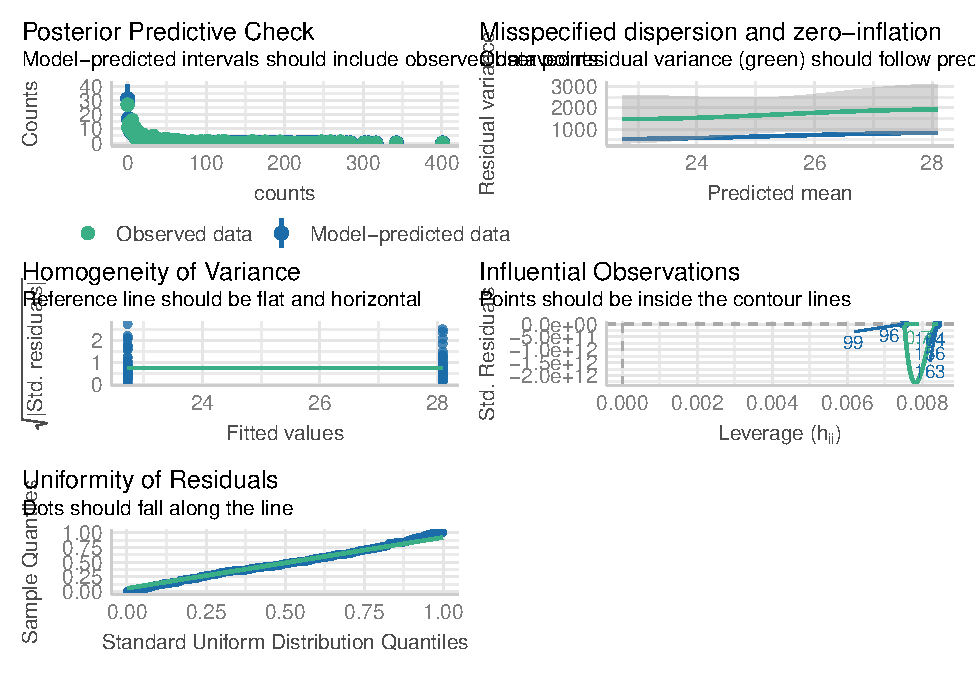
\includegraphics{hw1-lobstrs-eds241_files/figure-latex/unnamed-chunk-28-1.pdf}

\textbf{Comparison of m2\_pois \& m3\_nb}

The coefficient (0.2118) for the treatment variable as predicted by the
m3\_nb model tells us the change in the log-count of the outcome
(counts) for a one-unit increase in the treatment variable. Not only is
this a small change in the outcome/ a small treatment effect, but the
p-value for the treatment estimate is also not significant (0.218). This
indicates, according to m3\_nb, that the treatment does not appear to
have a strong influence in lobster counts.

The estimated coefficients of models m2\_pois and m3\_nb are very
similar. However, m2\_pois does not allow for zero-inflation and
overdispersion. On the other hand, m3\_nb tests did not detect
overdispersion and the zero-inflation test detected not an underfitting,
but rather a small OVERfitting of zeros.

Despite these encouraging m3\_nb results, the m3\_nb coefficient
p-values indicate that the model does not produce statistically
significant estimates. Thus, even if the negative binomial model makes
for a better fit, it does not allow us to confidently say that treatment
has an effect on lobster count.

\begin{center}\rule{0.5\linewidth}{0.5pt}\end{center}

Step 6: Compare models

\textbf{a.} Use the \texttt{export\_summ()} function from the
\texttt{jtools} package to look at the three regression models you fit
side-by-side.

\textbf{c.} Write a short paragraph comparing the results. Is the
treatment effect \texttt{robust} or stable across the model
specifications.

\begin{Shaded}
\begin{Highlighting}[]
\FunctionTok{export\_summs}\NormalTok{(m1\_ols, m2\_pois, m3\_nb,}
             \AttributeTok{model.names =} \FunctionTok{c}\NormalTok{(}\StringTok{"OLS"}\NormalTok{,}\StringTok{"Poisson"}\NormalTok{, }\StringTok{"NB"}\NormalTok{),}
             \AttributeTok{statistics =} \StringTok{"none"}\NormalTok{)}
\end{Highlighting}
\end{Shaded}

\begin{verbatim}
## Warning in (function (..., error_format = "({std.error})", error_pos = c("below", : Unrecognized statistics: none
## Try setting `statistics` explicitly in the call to `huxreg()`
\end{verbatim}

\begin{verbatim}
## Warning in build_tabular(ht): Multiple horizontal border widths in a single
## row; using the maximum.
\end{verbatim}

 
  \providecommand{\huxb}[2]{\arrayrulecolor[RGB]{#1}\global\arrayrulewidth=#2pt}
  \providecommand{\huxvb}[2]{\color[RGB]{#1}\vrule width #2pt}
  \providecommand{\huxtpad}[1]{\rule{0pt}{#1}}
  \providecommand{\huxbpad}[1]{\rule[-#1]{0pt}{#1}}

\begin{table}[ht]
\begin{centerbox}
\begin{threeparttable}
 \setlength{\tabcolsep}{0pt}
\begin{tabular}{l l l l}


\hhline{>{\huxb{0, 0, 0}{0.8}}->{\huxb{0, 0, 0}{0.8}}->{\huxb{0, 0, 0}{0.8}}->{\huxb{0, 0, 0}{0.8}}-}
\arrayrulecolor{black}

\multicolumn{1}{!{\huxvb{0, 0, 0}{0}}c!{\huxvb{0, 0, 0}{0}}}{\huxtpad{6pt + 1em}\centering \hspace{6pt}  \hspace{6pt}\huxbpad{6pt}} &
\multicolumn{1}{c!{\huxvb{0, 0, 0}{0}}}{\huxtpad{6pt + 1em}\centering \hspace{6pt} OLS \hspace{6pt}\huxbpad{6pt}} &
\multicolumn{1}{c!{\huxvb{0, 0, 0}{0}}}{\huxtpad{6pt + 1em}\centering \hspace{6pt} Poisson \hspace{6pt}\huxbpad{6pt}} &
\multicolumn{1}{c!{\huxvb{0, 0, 0}{0}}}{\huxtpad{6pt + 1em}\centering \hspace{6pt} NB \hspace{6pt}\huxbpad{6pt}} \tabularnewline[-0.5pt]


\hhline{>{\huxb{255, 255, 255}{0.4}}->{\huxb{0, 0, 0}{0.4}}->{\huxb{0, 0, 0}{0.4}}->{\huxb{0, 0, 0}{0.4}}-}
\arrayrulecolor{black}

\multicolumn{1}{!{\huxvb{0, 0, 0}{0}}l!{\huxvb{0, 0, 0}{0}}}{\huxtpad{6pt + 1em}\raggedright \hspace{6pt} (Intercept) \hspace{6pt}\huxbpad{6pt}} &
\multicolumn{1}{r!{\huxvb{0, 0, 0}{0}}}{\huxtpad{6pt + 1em}\raggedleft \hspace{6pt} 22.73 *** \hspace{6pt}\huxbpad{6pt}} &
\multicolumn{1}{r!{\huxvb{0, 0, 0}{0}}}{\huxtpad{6pt + 1em}\raggedleft \hspace{6pt} 3.12 *** \hspace{6pt}\huxbpad{6pt}} &
\multicolumn{1}{r!{\huxvb{0, 0, 0}{0}}}{\huxtpad{6pt + 1em}\raggedleft \hspace{6pt} 3.12 *** \hspace{6pt}\huxbpad{6pt}} \tabularnewline[-0.5pt]


\hhline{}
\arrayrulecolor{black}

\multicolumn{1}{!{\huxvb{0, 0, 0}{0}}l!{\huxvb{0, 0, 0}{0}}}{\huxtpad{6pt + 1em}\raggedright \hspace{6pt}  \hspace{6pt}\huxbpad{6pt}} &
\multicolumn{1}{r!{\huxvb{0, 0, 0}{0}}}{\huxtpad{6pt + 1em}\raggedleft \hspace{6pt} (3.57)\hphantom{0}\hphantom{0}\hphantom{0} \hspace{6pt}\huxbpad{6pt}} &
\multicolumn{1}{r!{\huxvb{0, 0, 0}{0}}}{\huxtpad{6pt + 1em}\raggedleft \hspace{6pt} (0.02)\hphantom{0}\hphantom{0}\hphantom{0} \hspace{6pt}\huxbpad{6pt}} &
\multicolumn{1}{r!{\huxvb{0, 0, 0}{0}}}{\huxtpad{6pt + 1em}\raggedleft \hspace{6pt} (0.12)\hphantom{0}\hphantom{0}\hphantom{0} \hspace{6pt}\huxbpad{6pt}} \tabularnewline[-0.5pt]


\hhline{}
\arrayrulecolor{black}

\multicolumn{1}{!{\huxvb{0, 0, 0}{0}}l!{\huxvb{0, 0, 0}{0}}}{\huxtpad{6pt + 1em}\raggedright \hspace{6pt} treat \hspace{6pt}\huxbpad{6pt}} &
\multicolumn{1}{r!{\huxvb{0, 0, 0}{0}}}{\huxtpad{6pt + 1em}\raggedleft \hspace{6pt} 5.36\hphantom{0}\hphantom{0}\hphantom{0}\hphantom{0} \hspace{6pt}\huxbpad{6pt}} &
\multicolumn{1}{r!{\huxvb{0, 0, 0}{0}}}{\huxtpad{6pt + 1em}\raggedleft \hspace{6pt} 0.21 *** \hspace{6pt}\huxbpad{6pt}} &
\multicolumn{1}{r!{\huxvb{0, 0, 0}{0}}}{\huxtpad{6pt + 1em}\raggedleft \hspace{6pt} 0.21\hphantom{0}\hphantom{0}\hphantom{0}\hphantom{0} \hspace{6pt}\huxbpad{6pt}} \tabularnewline[-0.5pt]


\hhline{}
\arrayrulecolor{black}

\multicolumn{1}{!{\huxvb{0, 0, 0}{0}}l!{\huxvb{0, 0, 0}{0}}}{\huxtpad{6pt + 1em}\raggedright \hspace{6pt}  \hspace{6pt}\huxbpad{6pt}} &
\multicolumn{1}{r!{\huxvb{0, 0, 0}{0}}}{\huxtpad{6pt + 1em}\raggedleft \hspace{6pt} (5.20)\hphantom{0}\hphantom{0}\hphantom{0} \hspace{6pt}\huxbpad{6pt}} &
\multicolumn{1}{r!{\huxvb{0, 0, 0}{0}}}{\huxtpad{6pt + 1em}\raggedleft \hspace{6pt} (0.03)\hphantom{0}\hphantom{0}\hphantom{0} \hspace{6pt}\huxbpad{6pt}} &
\multicolumn{1}{r!{\huxvb{0, 0, 0}{0}}}{\huxtpad{6pt + 1em}\raggedleft \hspace{6pt} (0.17)\hphantom{0}\hphantom{0}\hphantom{0} \hspace{6pt}\huxbpad{6pt}} \tabularnewline[-0.5pt]


\hhline{>{\huxb{0, 0, 0}{0.8}}->{\huxb{0, 0, 0}{0.8}}->{\huxb{0, 0, 0}{0.8}}->{\huxb{0, 0, 0}{0.8}}-}
\arrayrulecolor{black}

\multicolumn{4}{!{\huxvb{0, 0, 0}{0}}l!{\huxvb{0, 0, 0}{0}}}{\huxtpad{6pt + 1em}\raggedright \hspace{6pt}  *** p $<$ 0.001;  ** p $<$ 0.01;  * p $<$ 0.05. \hspace{6pt}\huxbpad{6pt}} \tabularnewline[-0.5pt]


\hhline{}
\arrayrulecolor{black}
\end{tabular}
\end{threeparttable}\par\end{centerbox}

\end{table}
 

\textbf{Comparing 3 models} The estimated treatment effects are similar
between m1\_ols, m2\_pois, and m3\_nb - when exponentiated, both m3\_nb
and m2\_pois estimate that the outcome will change by a factor of approx
1.236 (exp(0.2118)), or 23.6\% (1.236 − 1 = 0.236). m1\_ols has a
treatment coeff of 5.36, but when transformed to \% change, which is
(5.36/22.73)*100 = 23.6\%, we can clearly see that the estimated
treatment effect is basically the same across the 3 models.

Other than these similarities, the p-values of the estimated treatment
effects vary across models. In the OLS model the treatment coefficient
is not statistically significant. In the Poisson model the estimates are
statistically significant but tests revealed both overdispersion and
zero-inflation. Lastly, in the NB model tests showed no overdispersion
and only a slight overestimation of zero-inflation, but the estimates
were not statistically significant. When comparing the models, it is
clear that while the predicted treatment effect may appear stable across
models, it is not stable and not robust across different modeling
approaches.

\begin{center}\rule{0.5\linewidth}{0.5pt}\end{center}

Step 7: Building intuition - fixed effects

\textbf{a.} Create new \texttt{df} with the \texttt{year} variable
converted to a factor

\textbf{b.} Run the following negative binomial model using
\texttt{glm.nb()}

\begin{itemize}
\tightlist
\item
  Add fixed effects for \texttt{year} (i.e., dummy coefficients)
\item
  Include an interaction term between variables \texttt{treat} \&
  \texttt{year} (\texttt{treat*year})
\end{itemize}

\textbf{c.} Take a look at the regression output. Each coefficient
provides a comparison or the difference in means for a specific
sub-group in the data. Informally, describe the what the model has
estimated at a conceptual level (NOTE: you do not have to interpret
coefficients individually)

The model shows how the treatment effect is affected by the variable
`year', what the treatment effect was in the baseline year (2012). The
interaction term in this case aims at estimating how the treatment
effect changed over the years/how the difference in lobster counts
between MPAs and non-MPAs changed over the years. In general, the model
gives us a more complex and nuanced look at the mechanisms going on in
the data. In the baseline year, 2012, MPAs had significantly fewer
lobster than non-MPAs. This is also the year when these MPAs were
established. And, since lobster counts go up over the years in these MPA
sites, it shows that the treatment has had a positive effect on reef
sites even if the lobster counts of these aren't dramatically higher
than those of non-MPAs.

\textbf{d.} Explain why the main effect for treatment is negative? *Does
this result make sense?

This does make sense - the main effect for treatment is negative in the
baseline year (2012). In 2012, the lobster count in now-MPA sites was
lower because the benefits of the treatment were not yet tangible.

\begin{Shaded}
\begin{Highlighting}[]
\NormalTok{ff\_counts }\OtherTok{\textless{}{-}}\NormalTok{ spiny\_counts }\SpecialCharTok{\%\textgreater{}\%}
    \FunctionTok{mutate}\NormalTok{(}\AttributeTok{year=}\FunctionTok{as\_factor}\NormalTok{(year))}

\NormalTok{m5\_fixedeffs }\OtherTok{\textless{}{-}} \FunctionTok{glm.nb}\NormalTok{(}
\NormalTok{    counts }\SpecialCharTok{\textasciitilde{}}
\NormalTok{        treat }\SpecialCharTok{+}
\NormalTok{        year }\SpecialCharTok{+}
\NormalTok{        treat}\SpecialCharTok{*}\NormalTok{year,}
    \AttributeTok{data =}\NormalTok{ ff\_counts)}

\FunctionTok{summ}\NormalTok{(m5\_fixedeffs, }\AttributeTok{model.fit =} \ConstantTok{FALSE}\NormalTok{)}
\end{Highlighting}
\end{Shaded}

\begin{table}[!h]
\centering
\begin{tabular}{lr}
\toprule
\cellcolor{gray!10}{Observations} & \cellcolor{gray!10}{252}\\
Dependent variable & counts\\
\cellcolor{gray!10}{Type} & \cellcolor{gray!10}{Generalized linear model}\\
Family & Negative Binomial(0.8129)\\
\cellcolor{gray!10}{Link} & \cellcolor{gray!10}{log}\\
\bottomrule
\end{tabular}
\end{table}  \begin{table}[!h]
\centering
\begin{threeparttable}
\begin{tabular}{lrrrr}
\toprule
  & Est. & S.E. & z val. & p\\
\midrule
\cellcolor{gray!10}{(Intercept)} & \cellcolor{gray!10}{2.35} & \cellcolor{gray!10}{0.26} & \cellcolor{gray!10}{8.89} & \cellcolor{gray!10}{0.00}\\
treat & -1.72 & 0.42 & -4.12 & 0.00\\
\cellcolor{gray!10}{year2013} & \cellcolor{gray!10}{-0.35} & \cellcolor{gray!10}{0.38} & \cellcolor{gray!10}{-0.93} & \cellcolor{gray!10}{0.35}\\
year2014 & 0.08 & 0.37 & 0.21 & 0.84\\
\cellcolor{gray!10}{year2015} & \cellcolor{gray!10}{0.86} & \cellcolor{gray!10}{0.37} & \cellcolor{gray!10}{2.32} & \cellcolor{gray!10}{0.02}\\
\addlinespace
year2016 & 0.90 & 0.37 & 2.43 & 0.01\\
\cellcolor{gray!10}{year2017} & \cellcolor{gray!10}{1.56} & \cellcolor{gray!10}{0.37} & \cellcolor{gray!10}{4.25} & \cellcolor{gray!10}{0.00}\\
year2018 & 1.04 & 0.37 & 2.81 & 0.00\\
\cellcolor{gray!10}{treat:year2013} & \cellcolor{gray!10}{1.52} & \cellcolor{gray!10}{0.57} & \cellcolor{gray!10}{2.66} & \cellcolor{gray!10}{0.01}\\
treat:year2014 & 2.14 & 0.56 & 3.80 & 0.00\\
\addlinespace
\cellcolor{gray!10}{treat:year2015} & \cellcolor{gray!10}{2.12} & \cellcolor{gray!10}{0.56} & \cellcolor{gray!10}{3.79} & \cellcolor{gray!10}{0.00}\\
treat:year2016 & 1.40 & 0.56 & 2.50 & 0.01\\
\cellcolor{gray!10}{treat:year2017} & \cellcolor{gray!10}{1.55} & \cellcolor{gray!10}{0.56} & \cellcolor{gray!10}{2.77} & \cellcolor{gray!10}{0.01}\\
treat:year2018 & 2.62 & 0.56 & 4.69 & 0.00\\
\bottomrule
\end{tabular}
\begin{tablenotes}
\item Standard errors: MLE
\end{tablenotes}
\end{threeparttable}
\end{table}

\textbf{e.} Look at the model predictions: Use the
\texttt{interact\_plot()} function from package \texttt{interactions} to
plot mean predictions by year and treatment status.

\textbf{f.} Re-evaluate your responses (c) and (b) above.

The interactions plot supports my responses in c and d above.

\begin{Shaded}
\begin{Highlighting}[]
\NormalTok{ff\_counts}\SpecialCharTok{$}\NormalTok{predicted\_log }\OtherTok{\textless{}{-}} \FunctionTok{predict}\NormalTok{(m5\_fixedeffs, }\AttributeTok{type =} \StringTok{"link"}\NormalTok{)}
\NormalTok{ff\_counts}\SpecialCharTok{$}\NormalTok{predicted\_counts }\OtherTok{\textless{}{-}} \FunctionTok{exp}\NormalTok{(ff\_counts}\SpecialCharTok{$}\NormalTok{predicted\_log)}

\NormalTok{interact }\OtherTok{\textless{}{-}} \FunctionTok{ggplot}\NormalTok{(ff\_counts, }\FunctionTok{aes}\NormalTok{(}\AttributeTok{x =}\NormalTok{ year, }\AttributeTok{y =}\NormalTok{ predicted\_log, }\AttributeTok{color =}\NormalTok{ treat, }\AttributeTok{group =}\NormalTok{ mpa)) }\SpecialCharTok{+}
    \FunctionTok{geom\_line}\NormalTok{() }\SpecialCharTok{+}
    \FunctionTok{geom\_point}\NormalTok{() }\SpecialCharTok{+}
    \FunctionTok{labs}\NormalTok{(}\AttributeTok{y =} \StringTok{"Log of Counts"}\NormalTok{, }\AttributeTok{x =} \StringTok{"Year"}\NormalTok{) }\SpecialCharTok{+}
    \FunctionTok{theme\_minimal}\NormalTok{()}

\NormalTok{interact}
\end{Highlighting}
\end{Shaded}

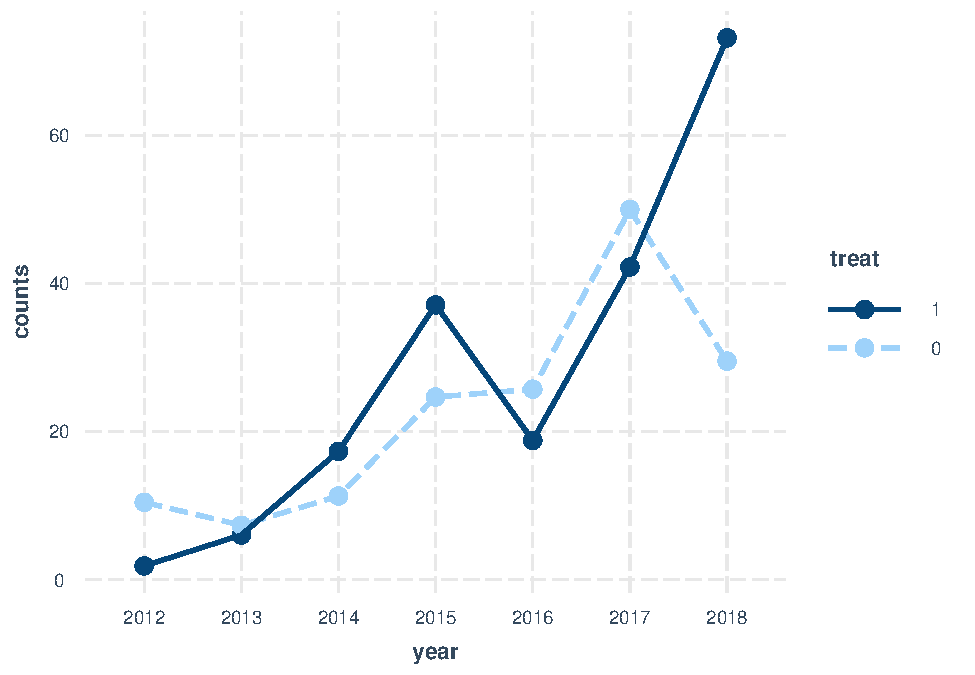
\includegraphics{hw1-lobstrs-eds241_files/figure-latex/unnamed-chunk-31-1.pdf}

\begin{Shaded}
\begin{Highlighting}[]
\CommentTok{\# HINT: Change \textasciigrave{}outcome.scale\textasciigrave{} to "response" to convert y{-}axis scale to counts}
\end{Highlighting}
\end{Shaded}

\textbf{g.} Using \texttt{ggplot()} create a plot in same style as the
previous \texttt{interaction\ plot}, but displaying the original scale
of the outcome variable (lobster counts). This type of plot is commonly
used to show how the treatment effect changes across discrete time
points (i.e., panel data).

The plot should have\ldots{} - \texttt{year} on the x-axis -
\texttt{counts} on the y-axis - \texttt{mpa} as the grouping variable

\begin{Shaded}
\begin{Highlighting}[]
\CommentTok{\# Hint 1: Group counts by \textasciigrave{}year\textasciigrave{} and \textasciigrave{}mpa\textasciigrave{} and calculate the \textasciigrave{}mean\_count\textasciigrave{}}
\CommentTok{\# Hint 2: Convert variable \textasciigrave{}year\textasciigrave{} to a factor}

\NormalTok{plot\_counts }\OtherTok{\textless{}{-}}\NormalTok{ spiny\_counts }\SpecialCharTok{\%\textgreater{}\%}
  \FunctionTok{group\_by}\NormalTok{(year, mpa) }\SpecialCharTok{\%\textgreater{}\%}
  \FunctionTok{summarize}\NormalTok{(}\AttributeTok{mean\_count =} \FunctionTok{mean}\NormalTok{(counts), }\AttributeTok{.groups =} \StringTok{"drop"}\NormalTok{) }\SpecialCharTok{\%\textgreater{}\%}
  \FunctionTok{mutate}\NormalTok{(}\AttributeTok{year =} \FunctionTok{as.factor}\NormalTok{(year))  }

\NormalTok{plot\_counts }\SpecialCharTok{\%\textgreater{}\%} \FunctionTok{ggplot}\NormalTok{(}\FunctionTok{aes}\NormalTok{(}\AttributeTok{x =}\NormalTok{ year, }
                           \AttributeTok{y =}\NormalTok{ mean\_count, }
                           \AttributeTok{group =}\NormalTok{ mpa, }\AttributeTok{color =}\NormalTok{ mpa)) }\SpecialCharTok{+}
  \FunctionTok{geom\_line}\NormalTok{(}\AttributeTok{size =} \DecValTok{1}\NormalTok{) }\SpecialCharTok{+}  
  \FunctionTok{geom\_point}\NormalTok{(}\AttributeTok{size =} \DecValTok{3}\NormalTok{) }\SpecialCharTok{+}
  \FunctionTok{labs}\NormalTok{(}
    \AttributeTok{title =} \StringTok{"Lobster counts over time by MPA status"}\NormalTok{,}
    \AttributeTok{x =} \StringTok{"Year"}\NormalTok{,}
    \AttributeTok{y =} \StringTok{"Mean lobster count"}\NormalTok{,}
    \AttributeTok{color =} \StringTok{"MPA status"}
\NormalTok{  ) }\SpecialCharTok{+}
  \FunctionTok{theme\_minimal}\NormalTok{() }\SpecialCharTok{+} 
  \FunctionTok{theme}\NormalTok{(}\AttributeTok{axis.text.x =} \FunctionTok{element\_text}\NormalTok{(}\AttributeTok{angle =} \DecValTok{45}\NormalTok{, }\AttributeTok{hjust =} \DecValTok{1}\NormalTok{)) }
\end{Highlighting}
\end{Shaded}

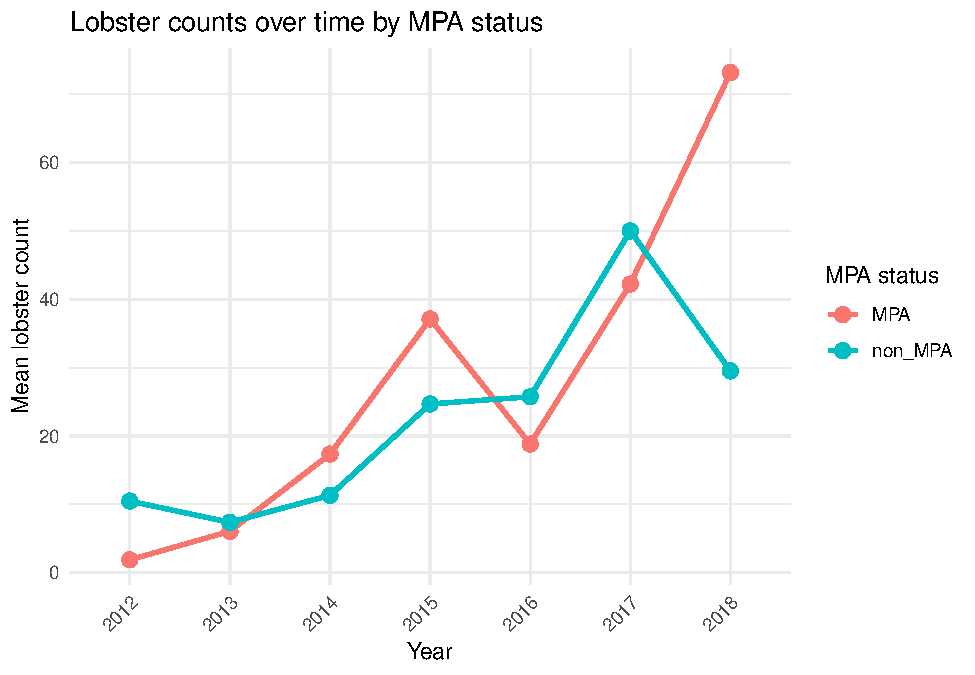
\includegraphics{hw1-lobstrs-eds241_files/figure-latex/unnamed-chunk-32-1.pdf}

\begin{center}\rule{0.5\linewidth}{0.5pt}\end{center}

Step 8: Reconsider causal identification assumptions

\begin{enumerate}
\def\labelenumi{\alph{enumi}.}
\tightlist
\item
  Discuss whether you think \texttt{spillover\ effects} are likely in
  this research context (see Glossary of terms;
  \url{https://docs.google.com/document/d/1RIudsVcYhWGpqC-Uftk9UTz3PIq6stVyEpT44EPNgpE/edit?usp=sharing})
\end{enumerate}

Yes, spillover effects are relevant in this research context. Lobster
can move without any limits between one MPA to another. When fishing
pressures change (in both MPAs and non), lobster respond to these
ecological and environmental changes in several ways - they may migrate
due to increased competition amongst them, they may move toward other
reefs due to temp changes, food availability etc.

\begin{enumerate}
\def\labelenumi{\alph{enumi}.}
\setcounter{enumi}{1}
\tightlist
\item
  Explain why spillover is an issue for the identification of causal
  effects
\end{enumerate}

The spillover effect is an issue for the identification of causal
effects because blurs the differences between treated and non-treated
reef sites. It complicates our ability to determine if the observed
changes in lobster populations are a result of treatment or of
unrelated/unintented lobster movement between reef sites.

\begin{enumerate}
\def\labelenumi{\alph{enumi}.}
\setcounter{enumi}{2}
\tightlist
\item
  How does spillover relate to impact in this research setting?
\end{enumerate}

Spillover can lead researchers to underestimate or overestimate the
efficacy of the treatment, leading to an inaccurate understanding of the
benefits of MPAs. Spillover can result in lobster counts being distorted
by the movement of lobsters between MPAs and non-MPAs. For example,
lower fishing pressure in MPAs could cause lobsters to migrate to
non-MPA areas where competition is lower, potentially inflating counts
in non-MPAs areas. Thus, spillover effects can distort the true impact
of MPAs on lobster populations, leading to biased estimates of their
effectiveness.

\begin{enumerate}
\def\labelenumi{\alph{enumi}.}
\setcounter{enumi}{3}
\item
  Discuss the following causal inference assumptions in the context of
  the MPA treatment effect estimator. Evaluate if each of the assumption
  are reasonable:

  \begin{enumerate}
  \def\labelenumii{\arabic{enumii})}
  \tightlist
  \item
    SUTVA: Stable Unit Treatment Value assumption
  \item
    Excludability assumption
  \end{enumerate}
\end{enumerate}

None of these assumptions are reasonable in the context of the MPA
treatment effect estimator. The SUTVA is more than likely violated by
the spillover effect since the changes in lobster count do not solely
depend on the treatment effect.The lobster count of a non-treated site
is affected by the treatment of another site. Furthermore, the treatment
is not applied in the exact same way across all treated reefs (MPAs) as
there are different levels of protection that an MPA can have. For
example, some MPAs like the one in Isla Vista are designated as
``no-take'' areas, but not all MPAs have this protection nor do they all
allow/prohibit the same activities.

Lastly, the excludability assumption is violated because other than the
spillover effect, there are countless other factors, human and and
non-human-related, that affect the health of reefs and the abundance of
lobster.

\begin{center}\rule{0.5\linewidth}{0.5pt}\end{center}

\section{EXTRA CREDIT}\label{extra-credit}

\begin{quote}
Use the recent lobster abundance data with observations collected up
until 2024 (\texttt{lobster\_sbchannel\_24.csv}) to run an analysis
evaluating the effect of MPA status on lobster counts using the same
focal variables.
\end{quote}

\begin{enumerate}
\def\labelenumi{\alph{enumi}.}
\tightlist
\item
  Create a new script for the analysis on the updated data
\item
  Run at least 3 regression models \& assess model diagnostics
\item
  Compare and contrast results with the analysis from the 2012-2018 data
  sample (\textasciitilde{} 2 paragraphs)
\end{enumerate}

\begin{center}\rule{0.5\linewidth}{0.5pt}\end{center}

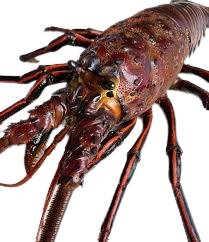
\includegraphics{figures/spiny1.png}

\end{document}
